\documentclass[
	a4paper
]{scrreprt}

%%% PACKAGES %%%

% PDF/A Compliance
\usepackage[a-2b,latxmp]{pdfx}

% add unicode support and use german as language
\usepackage[utf8]{inputenc}
\usepackage[ngerman]{babel}

% Use Helvetica as font
\usepackage[scaled]{helvet}
\renewcommand\familydefault{\sfdefault}
\usepackage[T1]{fontenc}

% Better tables
\usepackage{tabularx}

% Better enumerisation env
\usepackage{enumitem}

% Use graphics
\usepackage{graphicx}

% Have subfigures and captions
\usepackage{subcaption}

% Be able to include PDFs in the file
\usepackage{pdfpages}

% Have custom abstract heading
\usepackage{abstract}

% Need a list of equation
\usepackage{tocloft}
\usepackage{ragged2e}

% Better equation environment
\usepackage{amsmath}

% Symbols for most SI units
\usepackage{siunitx}

\usepackage{csquotes}

% Clickable Links to Websites and chapters
\usepackage{hyperref}

% Change page rotation
\usepackage{pdflscape}

% Symbols like checkmark
\usepackage{amssymb}
\usepackage{pifont}

\usepackage[absolute]{textpos}

% Glossary, hyperref, babel, polyglossia, inputenc, fontenc must be loaded before this package if they are used
\usepackage{glossaries}
% Redefine the quote charachter as we are using ngerman
\GlsSetQuote{+}
% Define the usage of an acronym, Abbreviation (Abbr.), next usage: The Abbr. of ...
\setacronymstyle{long-short}

% Bibliography & citing
\usepackage[
	backend=biber,
	style=apa,
	bibstyle=apa,
	citestyle=apa,
	sortlocale=de_DE
	]{biblatex}
\addbibresource{Referenzen.bib}
\DeclareLanguageMapping{ngerman}{ngerman-apa}

%%% COMMAND REBINDINGS %%%
\newcommand{\tabitem}{~~\llap{\textbullet}~~}
\newcommand{\xmark}{\ding{55}}
% Pro/Con item https://tex.stackexchange.com/questions/145198/change-the-bullet-of-each-item#145203
\newcommand\pro{\item[$+$]}
\newcommand\con{\item[$-$]}

% Define list of equations - Thanks to Charles Clayton: https://tex.stackexchange.com/a/354096
\newcommand{\listequationsname}{\huge{Formelverzeichnis}}
\newlistof{myequations}{equ}{\listequationsname}
\newcommand{\myequations}[1]{
	\addcontentsline{equ}{myequations}{\protect\numberline{\theequation}#1}
}
\setlength{\cftmyequationsnumwidth}{2.3em}
\setlength{\cftmyequationsindent}{1.5em}

% Usage {equation}{caption}{label}
% \indexequation{b = \frac{\pi}{\SI{180}{\degree}}\cdot\beta\cdot 6378.137}{Bogenlänge $b$ des Winkels $\beta$ mit Radius 6378.137m (Distanz zum Erdmittelpunkt am Äquator)}{Bogenlaenge}
\newcommand{\indexequation}[3]{
	\begin{align} \label{#3} \ensuremath{\boxed{#1}} \end{align}
	\myequations{#3} \centering \small \textit{#2} \normalsize \justify }

% Todolist - credit to https://tex.stackexchange.com/questions/247681/how-to-create-checkbox-todo-list
\newlist{todolist}{itemize}{1}
\setlist[todolist]{label=$\square$}

% Nested Enumeratelist credit to https://tex.stackexchange.com/a/54676
\newlist{legal}{enumerate}{10}
\setlist[legal]{label*=\arabic*.}

%%% PATH DEFINITIONS %%%
% Define the path were images are found
\graphicspath{{./img/}{./appendix/}}

%%% GLOSSARY ENTRIES %%%
\makeglossaries
\newacronym{RFID}{RFID}{Radio-Frequency Identification}
\newglossaryentry{HF}{name={HF},description={High Frequency, RFID Tags im Frequenzbereich von 3-30MHz}}
\newglossaryentry{UHF}{name={UHF},description={Ultra High Frequency, RFID Tags im Frequenzbereich von 0.3-30GHz}}
\newglossaryentry{DLL}{name={DLL},description={Dinamic Link Library, eine dynamisch ladbare Programmbibliothek}}

%%% DOCUMENT %%%

\begin{document}

%%% Fallback DocumentVersion if Builded local
\providecommand{\docversion}{0.0-localBuild}
\begin{titlepage}
	\begin{textblock*}{5cm}[0,0](15.1cm,1cm)
		
\includegraphics[keepaspectratio,width=5cm]{img/HSLU_Logo}
	\end{textblock*}
	\begin{center}
		\vspace*{5cm}
		\Huge{\textbf{Suche von mit RFID ausgerüsteten Einzelexemplaren im vollautomatischen Behälter-Hochregallager}} \\
		\vspace{0.5em}
		\Large{Bachelordiplomarbeit FS2019}\\
		\vspace{3em}
		\LARGE{Pascal Baumann, Dane Wicki}\\
		\vspace{1em}
		\Large{Betreuer: Martin Jud}\\
		\vfill
		\large{Hochschule Luzern - Departement Informatik}\\
		\large{\today}\\
		\large{Version \docversion}
	\end{center}
	\begin{textblock*}{5cm}[0,0](15.3cm,277mm)
		
\includegraphics[keepaspectratio,width=5cm]{img/FHZ_Logo}
	\end{textblock*}
\end{titlepage}

\newpage

\pagenumbering{gobble}

\begin{textblock*}{5cm}[0,0](15cm,0.7cm)
	
\includegraphics[keepaspectratio,width=2.7cm]{img/HSLU_Logo_Header}
\end{textblock*}

\vspace*{1.35cm}

\noindent
\textbf{\Large{Bachelorarbeit an der Hochschule Luzern - Informatik}}

\vspace{0.6cm}
\noindent
\textbf{Titel:} RFID markierte Exemplare

\vspace{0.6cm}
\noindent
\textbf{Student 1:} Pascal Baumann

\vspace{0.6cm}
\noindent
\textbf{Student 2:} Dane Wicki

\vspace{1cm}
\noindent
\textbf{Studiengang:} BSc Informatik

\vspace{0.6cm}
\noindent
\textbf{Abschlussjahr:} 2019

\vspace{0.6cm}
\noindent
\textbf{Betreuungsperson:} Martin Jud

\vspace{0.6cm}
\noindent
\textbf{Experte:} Urs Gehrig

\vspace{0.6cm}
\noindent
\textbf{Codierung / Klassifizierung der Arbeit:}

\begin{todolist}
	\item \textbf{A: Einsicht (Normalfall)}
	\item \textbf{B: Rücksprache}\hspace*{0.7cm}(Dauer:\hspace*{1cm} Jahr / Jahre)
	\item \textbf{C: Sperre}\hspace*{1.865cm}(Dauer:\hspace*{1cm} Jahr / Jahre)
\end{todolist}

\vfill

\noindent
\textbf{Eidesstattliche Erklärung}
\\
Ich erkläre hiermit, dass ich/wir die vorliegende Arbeit selbständig und ohne unerlaubte fremde Hilfe angefertigt haben, alle verwendeten Quellen, Literatur und andere Hilfsmittel angegeben haben, wörtlich oder inhaltlich entnommene Stellen als solche kenntlich gemacht haben, das Vertraulichkeitsinteresse des Auftraggebers wahren und die Urheberrechtsbestimmungen der Fachhochschule Zentralschweiz (siehe Markblatt «Studentische Arbeiten» auf MyCampus) respektieren werden.

\vspace{1em}

\noindent
\begin{tabularx}{\textwidth}{@{}lX}
	&\\
	Ort / Datum, Unterschrift: &  \\
	\cline{2-2}
	&\\[0.5cm]
	Ort / Datum, Unterschrift: &  \\
	\cline{2-2}
\end{tabularx}

\begin{textblock*}{5cm}[0,0](14.93cm,277mm)
	
\includegraphics[keepaspectratio,width=5cm]{img/FHZ_Logo}
\end{textblock*}

\newpage

\begin{textblock*}{5cm}[0,0](15cm,0.7cm)
	
\includegraphics[keepaspectratio,width=2.7cm]{img/HSLU_Logo_Header}
\end{textblock*}

\noindent
\textbf{Abgabe der Arbeit auf der Portfolio Datenbank}

\vspace{0.5em}

\noindent
\textbf{Bestätigungsvisum Studentin / Student}
\\
\noindent
Ich bestätige, dass ich die Bachelorarbeit korrekt gemäss Merkblatt auf der Portfolio Datenbank abgelegt habe. Die Verantwortlichkeit sowie die Berechtigungen habe ich abgegeben, so dass ich keine Änderungen mehr vornehmen kann oder weitere Dateien hochladen kann.

\vspace{0.7em}

\noindent
\begin{tabularx}{\textwidth}{@{}lX}
	&\\
	Ort / Datum, Unterschrift: &  \\
	\cline{2-2}
	&\\[0.5cm]
	Ort / Datum, Unterschrift: &  \\
	\cline{2-2}
\end{tabularx}

\vspace{0.8cm}
\noindent
\textbf{Verdankung}
\\
An dieser Stelle möchten wir uns bei all denjenigen bedanken, die uns bei der Erstellung dieser Bachelorarbeit unterstützt haben. Als Erstes möchten wir uns bei unserem Betreuer Martin Jud bedanken, der unsere Bachelorarbeit unterstützt und begutachtet hat. Für die hilfreichen Empfehlungen zur Struktur dieser Arbeit und den Hilfestellungen zur Anschaffung der Versuchshardware möchten wir uns herzlich bedanken. Weiter möchten wir uns bei Urs Gehrig für seinen Einsatz als Experten für unsere Arbeit bedanken. Einen Dank auch an Herrn Mike Märki, welcher diese Arbeit überhaupt erst ermöglicht hat, und uns erlaubte unsere Referenzimplementation vor Ort zu testen. Ganz herzlich möchten wir uns auch bei Jeremy Meier bedanken, welcher uns in der Architektur beraten und ein Review der Systemspezifikation geliefert hat. Einen herzlichen Dank auch an Herrn Andreas Sieber, welcher unsere Arbeit gegenlas und Korrekturvorschläge anbrachte.

\vspace{0.8cm}
\noindent
\textbf{Eingangsvisum (durch das Sekretariat auszufüllen):}

\noindent
\renewcommand{\arraystretch}{2}
\begin{tabularx}{\textwidth}{@{}lXlX}
	Rotkreuz, den & & Visum: & \\
	\cline{2-2}
	\cline{4-4}
\end{tabularx}
\renewcommand{\arraystretch}{1}

% Uncomment for print_version

% \vfill
% \noindent
% \textbf{Hinweis}: Die Bachelorarbeit wurde von keinem Dozierenden nachbearbeitet. Veröffentlichungen (auch auszugsweise) sind ohne das Einverständnis der Studiengangleitung der Hochschule Luzern – Informatik nicht erlaubt.

% \vspace{1em}
% 
% \noindent
% \textbf{Copyright} © 2019 Hochschule Luzern - Informatik
% 
% \vspace{1em}
% \noindent
% Alle Rechte vorbehalten. Kein Teil dieser Arbeit darf ohne die schriftliche Genehmigung der Studiengangleitung der Hochschule Luzern - Informatik in irgendeiner Form reproduziert oder in eine von Maschinen verwendete Sprache übertragen werden.

\begin{textblock*}{5cm}[0,0](14.93cm,277mm)
	
\includegraphics[keepaspectratio,width=5cm]{img/FHZ_Logo}
\end{textblock*}


\pagenumbering{Roman}

\renewcommand{\abstractname}{Management Summary}
\begin{abstract}
	Abstract
\end{abstract}

\tableofcontents

\clearpage
\pagenumbering{arabic}

\chapter{Einleitung}
\label{ch:Einleitung}
In der Kooperativen Speicherbibliothek Schweiz werden Exemplare der dem Verein zugehörigen Bibliotheken eingelagert. Das heisst, das Exemplar der Bibliothek wird gereinigt und inventarisiert eingelagert. Sollte ein Bibliotheksbenutzer ein Exemplar dieses Werks anfordern, wird das Exemplar per Kurier an die jeweilige Bibliothek verschickt. Journale oder Magazine werden vorzugsweise eingescannt und in digitaler Form an den Benutzer übergeben, sofern dies so vom Benutzer bestellt wurde. Sowohl die beteiligten Bibliotheken, wie auch die Bibliotheksbenutzer sind daher an einer zeitgerechten Lieferung interessiert. Dies bedeutet für die Speicherbibliothek, dass alle Prozesse und Abläufe effizient und zuverlässig ablaufen müssen. Verzögerungen in Zwischenschritten können sich auf die ganze Auslieferung des Exemplars, in physischer oder digitaler Form, auswirken.

Im Hochregallager der Speicherbibliothek werden momentan bis zu 110'000 Behältern mit verschiedenen Exemplaren, von welchen viele mit RFID Tags ausgestattet sind, gelagert. Die Behälter werden manuell von Menschen befüllt und entleert, und anschliessend voll autonom an einen Lagerplatz gefahren. Zeitweise können auch gewisse Exemplare wieder aus den Behältern entnommen werden, um dieses Exemplar zu Lesen, Scannen, der teilnehmenden Bibliotheken zurückzusenden, oder aus dem Lagerbestand zu entfernen. Der Vorgang des Lagern und Entnehmens birgt die Gefahr, dass eine Person aus Versehen ein Exemplar in einen falschen Behälter einsortiert. Dies führt zu dem Umstand, dass das Exemplar nur sehr umständlich wiedergefunden werden kann \parencite{WickiBaumann2019Projektbeschrieb}.

In dieser Arbeit wird daher eine Lösung für das Problem der Deplatzierung als Konzept ausgearbeitet, dieses Konzept in einer Machbarkeitsstudie geprüft und mit einer Referenzimplementation validiert.

\section{Aufgabenstellung und Zielsetzung}
Ziel dieser Arbeit ist es, mittels einer Machbarkeitsstudie und einem Proof of Concept zu untersuchen, ob es technisch realisierbar ist, Exemplare, welche mit RFID Tags ausgerüstet sind, im Hochregallager der Speicherbibliothek zu finden \parencite{WickiBaumann2019Projektbeschrieb}.

Daraus leiteten sich die folgenden Artefakte ab, welche dem Kunden abgegeben werden:
\begin{itemize}
	\item Zwei ausgearbeiteten Konzepte
	\item Eine Machbarkeitsstudie zu einem ausgewählten Konzept
	\item Ein Versuchsprotokoll, basiernd auf den vor Ort durchgeführten Versuchen
\end{itemize}


\chapter{Stand der Technik}
\label{ch:StandDerTechnik}

Das erste \gls{RFID}-System wurde von den Allierten im Zweiten Weltkrieg eingesetzt. Deren Freund-Feind-Erkennung funktionierte über eine passive Reflektion der Radarwellen, welche auf die Frequenz der Radarsender geeicht war. Verbündete Flieger ergaben dadurch ein viel stärkeres Signal und waren als hellere Punkte erkennbar (\cite{chawla2007}, \cite{uswardep1946_3}). In den 1960er wurden in den USA verschiedenste Patente angemeldet, welche sich das Prinzip der elektromagnetischen Induktion zunutze machen, um sich gegenüber einem Sender zu identifizieren. Die Adaption der Technologie liess jedoch auf sich warten, \citeauthor{want2004} identifiziert als Grund dafür die fehlende Marktviabilität, die Ausgereiftheit der Technologie selbst und die Adaptionskosten \parencite{want2004}. All dies hat sich in den 60 Jahren seither geändert und \gls{RFID} ist eine etablierte Technologie, welche in verschiedensten Sparten eingesetzt wird.

\section{Technologische Grundlagen}

Ein \gls{RFID} System besteht generell aus zwei Teilen: Einem Sender und Empfänger, diese werden Interrogator (dt. Anfragender) und Transponder (dt. Sendegerät) genannt. Der Transponder wird auch als \gls{RFID} Tag bezeichnet und kann sowohl passiv, das heisst ohne Stromversorgung auf dem Tag, wie auch aktiv sein, das heisst der Chip und die Antenne werden durch eine integrierte Batterie versorgt. Der Vorteil eines aktiven Tags liegt in dessen höherer Reichweite. Als Mischung zwischen den Beiden ist der semi-aktive Tag, bei dem nur der Chip durch die Batterie mit Energie versorgt wird, und die Antenne durch das Feld des Interrogators gespiesen wird.

Bei der Funktionsweise von \gls{RFID} Tags muss man zwischen zwei Funktionalitäten unterscheiden, welche auf die Entfernung zwischen Transponder und Interrogator abhängig sind. Im Nahbereich (engl. Near-Field \gls{RFID}) funktioniert die Stromversorgung über magnetische Induktion (die Arbeitsspannung der Chips liegt im Mikro- bis Miliwattbereich). Die Kommunikation zwischen Interrogator und Transponder wird über "load modulation"\ realisiert. Dies bedeutet, dass der Transponder, aktiviert durch das Feld des Interrogator, selber beginnt ein Feld auszustrahlen. Dadurch entstehen Interferenzen im Feld welche sich durch minimale Spannungsänderungen in der Spule des Interrogators messen lassen \parencite{want2006}. Die Distanz des Nahfelds ist durch die Gleichung \ref{NearFieldEM} gegeben. Für \gls{HF} Tags (wie diejenigen die auch in der Speicherbibliothek verwendet werden) ist die Betriebsfrequenz durch den ISO Standard 18000-3 auf 13.56MHz festgelegt und ergibt damit eine Distanz von 3.519m für das Nahfeld.

\indexequation{d=\frac{\lambda}{2\pi}}{Reichweite des reaktiven Nahfelds}{NearFieldDistance}
\indexequation{\lambda=\frac{c}{f}}{Definition der Wellenlänge $\lambda$ in Abhängigkeit der Lichtgeschwindigkeit c}{Wavelength}
\indexequation{d=\frac{c}{2\lambda\pi}}{Definition der Wellenlänge in Gleichung \ref{NearFieldDistance} eingesetzt}{NearFieldEM}

Im Fernfeldbereich erhält der \gls{RFID} Tag direkt über die ausgestrahlte Elektromagnetischen Wellen. Die Abnahme der Energiedichte auf Distanz ist dabei proportional zu $\frac{1}{r^2}$. Dennoch ist es durch Fortschritte in der Miniaturisierung und besserer Energieeffizienz moderner Halbleiter und Chips möglich dadurch \gls{UHF} Tags mit Strom zu versorgen. Die Kommunikation funktioniert mittels "back scattering"\ - eine Antenne welche auf eine bestimmte Frequenz eingestellt ist, absorbiert den Grossteil der Wellen die gesendet werden. Passt jedoch die Impedanz nicht genau, so reflektiert die Antenne ein Teil des Signals an die Quelle, den Interrogator, zurück. Durch das Anpassen der Impedanz der Antenne über die Zeit, kann mehr oder weniger des Signals reflektiert und so eine Nachricht codiert werden \parencite{want2006}.

\begin{figure}[htb]
	\centering
	\begin{subfigure}[b]{0.8\linewidth}
		\centering
		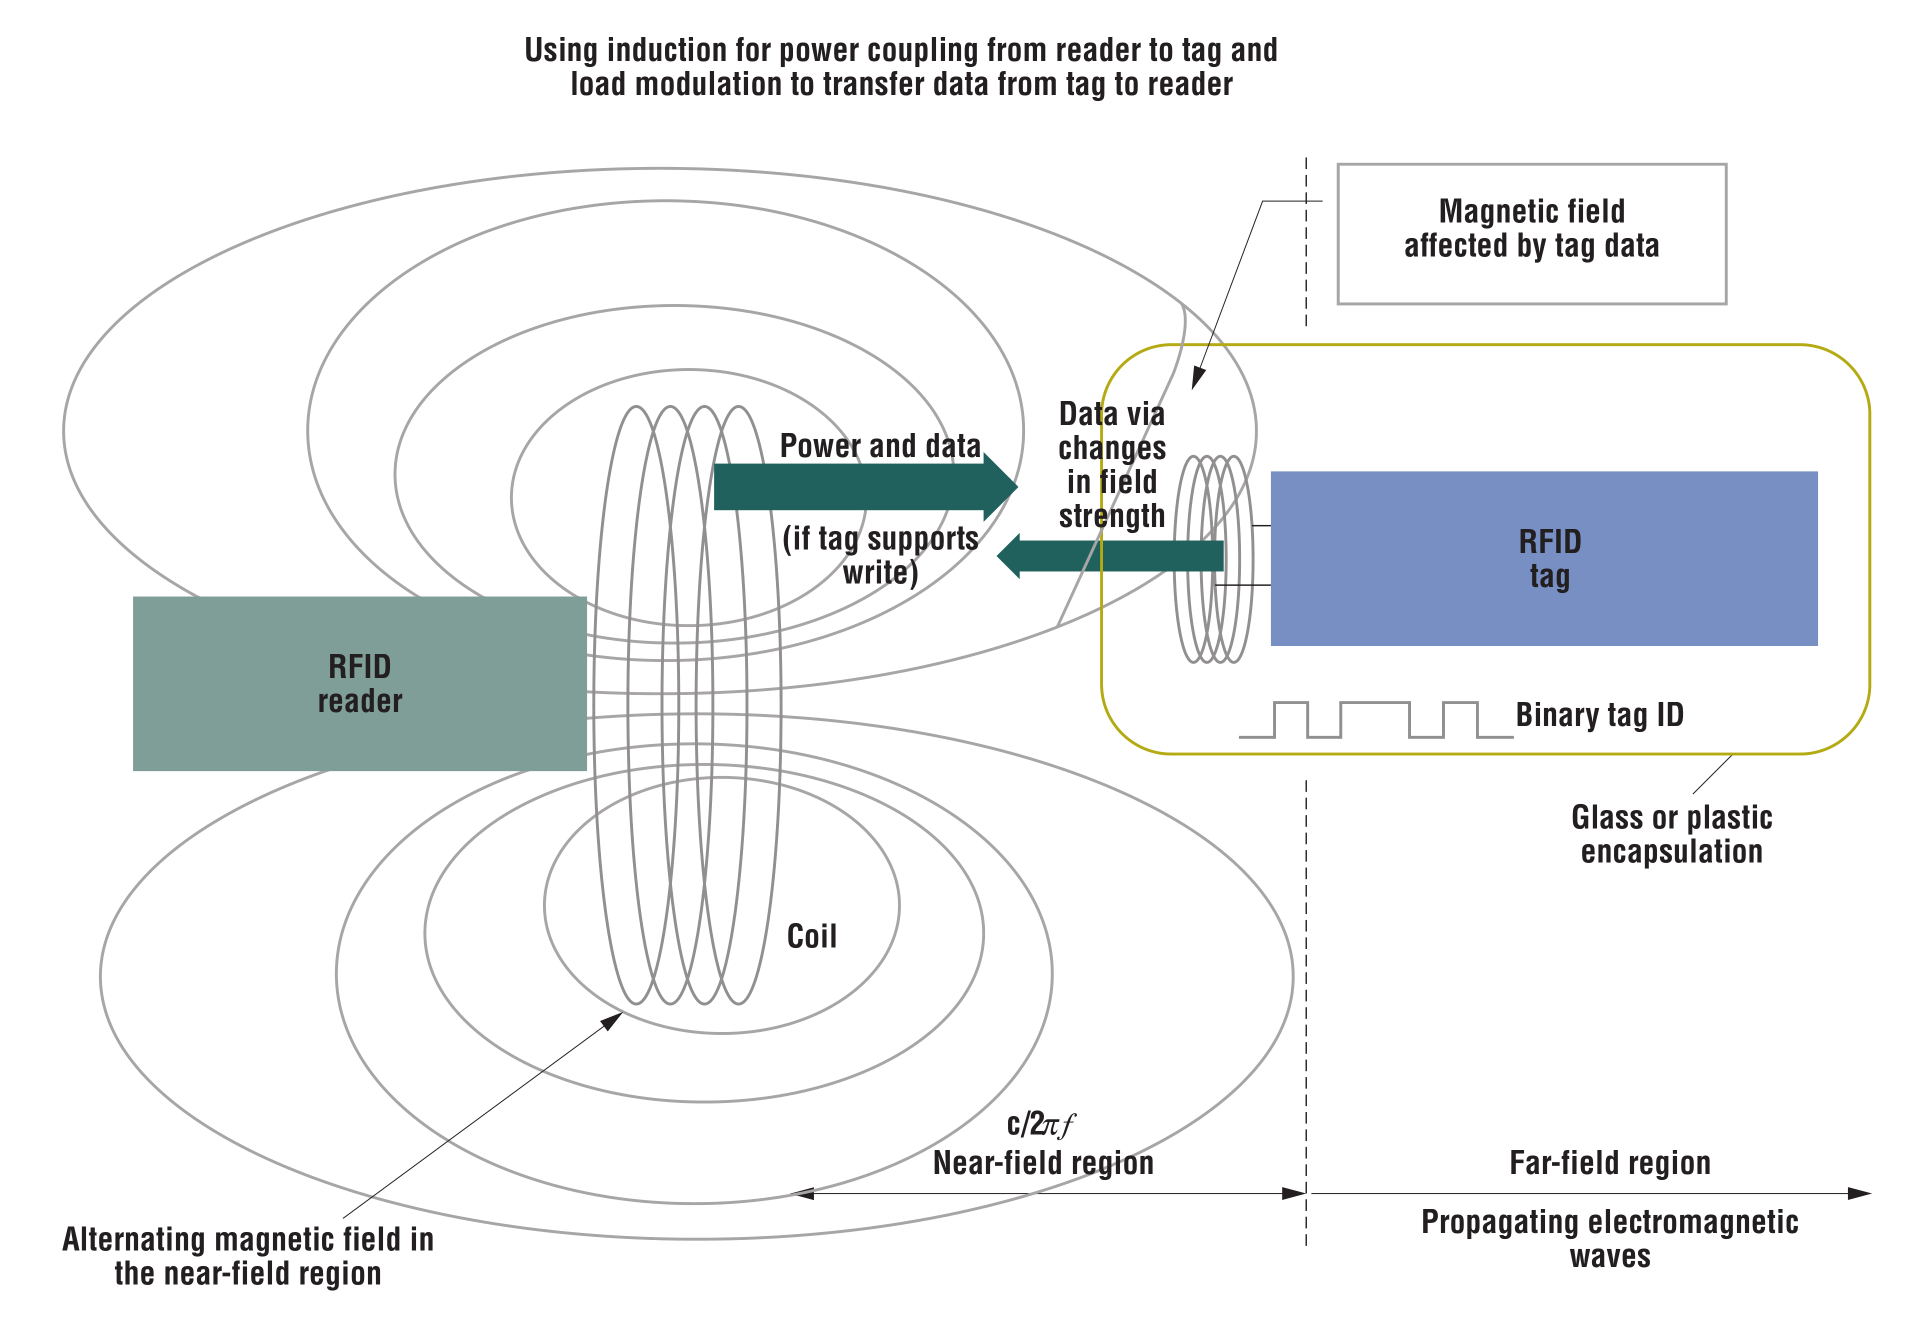
\includegraphics[keepaspectratio,width=\linewidth]{InductionCoupling}
		\caption{Magnetische Induktion und "load modulation"}
	\end{subfigure}
	\begin{subfigure}[b]{0.8\linewidth}
		\centering
		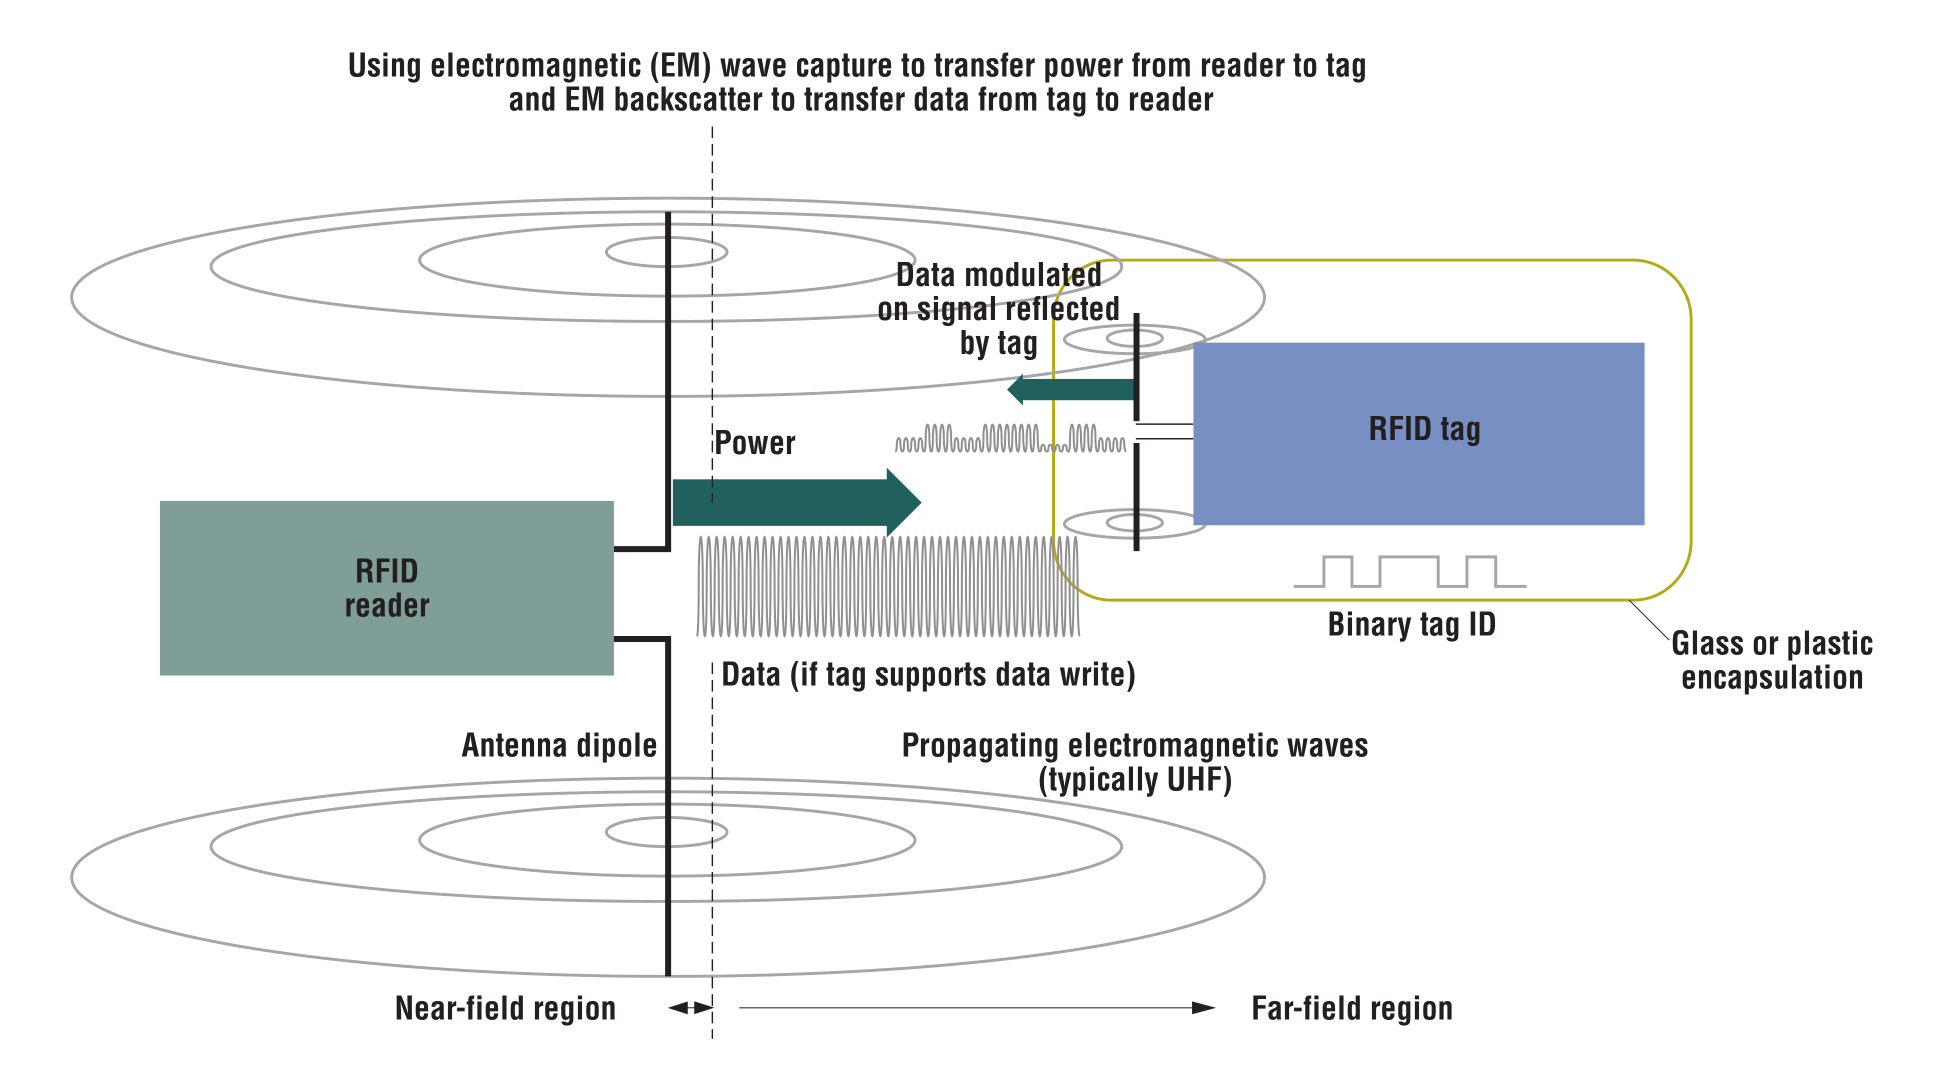
\includegraphics[keepaspectratio,width=\linewidth]{Backscattering}
		\caption{EM Wellentransmission und "backscattering"}
	\end{subfigure}
	\caption{Funktionsweisen von Nah- und Fernfeld \gls{RFID} Tags graphisch dargestellt \parencite{want2006}}
\end{figure}

\section{Technische Konzepte}

Da auf eine Anfrage eines Interrogators alle Chips in dessen Nähe antworten, ist der Luft\-raum daher als eine Kollisionsdomäne zu verstehen. Dies bedeutet, dass alle beteiligten Parteien auf dem gleichen Medium sind, sich also gegenseitig stören können. Dieses Problem kennt man in der Netzwerktechnik seit Tokenring, und heutzutage vor allem im WLAN Bereich. Die bei \gls{RFID} verwendete Strategie ist dabei die Kollisionsvermeidung und funktioniert nach dem folgenden Prinzip:
\begin{enumerate}
	\item Ein Tag sendet nur nach Empfang der kompletten Befehlssequenz des Interrogator
	\item Ein Tag sendet nur falls er spezifisch angefragt wurde
\end{enumerate}
Der Interrogator unterteilt daher während einer Inventur seine Anfrage in unterschiedliche Zeitbereiche. Pro Bereich fragt er nach den Identifikationsnummern von Tags mit einer Maske, diese Antworten nur falls die Maske auf Ihre Identifikationsnummer passt. Geschieht dabei eine Kollision, so wird der betreffende Bereich weiter unterteilt, bis das ganze Inventar erfasst wurde \parencite{ISO15693-3}.

Für \gls{RFID} sind in den ISO Diskussionen verschiedene Frequenzen festgelegt worden. Diese bieten unterschiedliche Vor- und Nachteile welche in der Tabelle \ref{tbl:RFIDFrequencies} dargestellt werden.

\begin{table}[htb]
	\begin{tabularx}{\textwidth}{|X|X|X|X|X|}
		\hline
		\textbf{Frequenz\-bereich} & \textbf{LF (< 135kHz)} & \textbf{HF (13.56MHz)} & \textbf{UHF (860-960MHz)} & \textbf{Mikrowelle (2.45GHz)}\\
		\hline
		\textbf{Lesereichweite} & <0.5m & \textasciitilde 1m & \textasciitilde 4-5m & \textasciitilde 1m\\
		\hline
		\textbf{Typ} & passiv & passiv & passiv oder aktiv & passiv oder aktiv\\
		\hline
		\textbf{Parallele Leserate} & langsam & langsam & schnell & schnell \\
		\hline
		\textbf{Interferenz durch Wasser und Metal} & wenig & wenig & viel & viel \\
		\hline
		\textbf{Grösse der Tags} & gross & gross & klein & klein \\
		\hline
	\end{tabularx}
	\caption{Vor- und Nachteile der unterschiedlichen Betriebsfrequenzen von \gls{RFID} Tags \parencite{chawla2007}}
	\label{tbl:RFIDFrequencies}
\end{table}


\chapter{Methode}

\section{Projektinformationen}

\subsection{Vorgehensmodell}

Alle Wirtschaftsprojekte an der Hochschule Luzern fallen in eine der folgenden Kategorien:

\begin{enumerate}
	\item Einsatz von Standardsoftware und Services
	\item Software- und Produktentwicklung
	\item Innovationsprojekt
	\item IT-Infrastrukturentwicklung
	\item Strukturierte Analyse und Konzeption von Systemen und Abläufen
\end{enumerate}

Dabei ist dieses Projekt als Innovationsprojekt und Softwareentwicklung klassifiziert worden. Wir erwarteten daher unter anderem, eine Evaluation, Recherchen und weitere Unbekannten. Um auf diese eingehen zu können, entschied sich das Team dafür die hybride, inkrementelle Agile Methode zu verwenden.

\subsection{Agile Projektmethode}

Die agile Projektmethode zielt darauf ab in einem ungewissen und sich verändernden Umfeld zu bestehen. Insbesondere bedeutet dies, das auf sich verändernde Voraussetzungen schnell reagiert werden kann und dabei ein funktionierendes Produkt entsteht \parencite{AgileAlliance2015}. Dies soll durch eine enge Zusammenarbeit mit dem Auftraggeber und guter teaminterner Kommunikation erreicht werden.

\parencite{BaumannWicki2018}

\subsection{Ermittlung offener Projektrahmenbedingungen}
\label{ch:evaluation}

\subsection{Projektanforderungen}
Mittels einer Machbarkeitsstudie und einem Proof of Concept soll untersucht werden ob es möglich ist bis zu 120 \gls{RFID} Tags in einem Behälter mit der Dimension 600x400x320mm zu identifizieren.

\begin{legal}
	\item Es sollen mindestens zwei Lösungskonzepte für eine als Auswahl der Machbarkeitsstudie entwickelt werden.
	\item Die Lösungskonzepte müssen auf deren technische Realisierbarkeit untersucht werden.
	\item Es muss mindestens ein entwickeltes Konzept für die Machbarkeitsstudie verwendet werden.
	\item Die Machbarkeitsstudie muss eine Kostenrechnung für die Lösungsansätze beinhalten.
	\item Es soll eine Referenzimplementation entwickelt werden, welche vom Kunde verwendet werden kann.
	
	\item Anforderungen an Konzepte
	\begin{legal}
		\item Die Lösungskonzepte müssen mit dem Lagersystem kommunizieren können
		\item Die Lösungskonzepte müssen die RFID Tags in weniger als 1 Sekunden identifizieren können.
		\item Die Lösungskonzepte müssen für das bestehende Hochregallager der Speicherbibliothek verwendbar sein.
	\end{legal}
	\item Anforderungen an Proof of Concept
	\begin{legal}
		\item Das Proof of Concept muss technisch aufzeigen, wie viele RFID Tags in einer Sekunde identifiziert werden können.
	\end{legal}
	\item Anforderungen an Referenzimplementation
	\begin{legal}
		\item Die Referenzimplementation soll mit einer Oracle Datenbank kommunizieren können.
		\item Die Referenzimplementation ist in der Lage die Buch ID eines Exemplares über RFID auszulesen.
		\item Die Referenzimplementation soll erkennen, wenn eine Box ein Exemplar (eines, welches mit RFID ausgestattet ist und technisch auch Lesbar ist) enthält, welches nicht dieser Box zugehörig ist.
		\item Die Referenzimplementation soll jede Unstimmigkeit (Exemplar, welches nicht zu diesem Behälter gehört) in einem Logdokument persistieren.
		\item Die Referenzimplementation soll in der Lage sein, dem Endbenutzer, in graphischer Form durch eine Konsolen-Ausgabe, mitzuteilen, welcher Behälter eine Unstimmigkeit enthält.
		\item Die Referenzimplementation soll die unter Laborbedingungen erhaltenen Resultate unter Realbedingungen verifizieren.
	\end{legal}
\end{legal}

\subsection{Einschränkungen und Abgrenzungen}
Um die Konzepte sowie Versuche vor Ort zu validieren, wurde eine Referenzimplementation entwickelt. Diese zu einer Produktionsreife zu bringen, war explizit nicht Teil des Projektes. Zur Entwicklung der Referenzimplementation wurde ein Datenbankauszug verwendet, und nicht eine Schnittstelle zur real verfügbaren Datenbank. Die Entwicklung einer produktionsreifen Applikation wurde in der Planung des Folgeprojektes, im Rahmen der Machbarkeitsstudie, berücksichtigt. Auf die Form dieser Applikation wurde jedoch nicht genauer eingegangen, sodass diese Spezifikation im Ermessen des nächsten Projektteames liegt.

Einschränkungen ergaben sich durch das beschränkte Budget, wodurch auf einen alternativen Hersteller ausgewichen werden musste, welcher eine kleinere Reichweite als gewünscht lieferte. Die Resultate können daher auch nur explizit für diese spezifische Hardware gewährleistet werden.
Weiter bestand Teamintern ein kleiner Wissensstand über die Durchführung einer Machbarkeitsstudie zu Beginn des Projektes, welcher im Laufe des Projektes zuerst erarbeitet werden musste.

\section{Machbarkeitsstudie}
Die Machbarkeitsstudie diente dazu ein ausgewähltes Konzept zu validieren und auf deren Machbarkeit zu untersuchen. Insbesondere wurde auf die technische und wirtschaftliche Machbarkeit wert gelegt. Da die Erarbeitung einer Machbarkeitsstudie eine Neuheit für beide Teammitglieder war, wurde zuerst in einer Recherchenphase offene Fragen geklärt. Dabei wurde eine Anleitung zur Erarbeitung einer Machbarkeitsstudie erstellt (siehe Kapitel \ref{app:ch:AnleitungMachbarkeitsstudie}). Diese stützt sich in grossen Teilen auf eine Anleitung des US Departement of Agriculture \parencite{Matson2000}.


\chapter{Ideen und Konzepte}

\section{Grundidee}

\section{Lösungskonzept 1}

\section{Lösungskonzept 2}


\chapter{Realisierung}

\section{Technische Erkenntnisse}

\subsection{Blöcke auf dem Chip}
Durch Auslesen mehrerer ausgeliehenen Büchern und dem Abgleich mit der erhaltenen Datenbank von der Speicherbibliothek, wurde herausgefunden, dass die Blöcke null bis drei die für die Buch-ID relevanten Informationen enthalten (siehe Tabelle \ref{tbl:ListeBloecke} und Abbildung \ref{fig:AusgeleseneBloeckeUndBarcode}). Weiter werden für die ID des Buches nur darstellbare Unicode-Charaktere verwendet und nicht der geschriebene Hex-Code.

\begin{table}[htb]
	\begin{tabularx}{\textwidth}{|l|l|l|X|}
		\hline
		\textbf{Blocknummer} & \textbf{Inhalt (Hex)} & \textbf{Inhalt (UTF8)} & \textbf{Beschreibung}\\
		\hline
		0 & 11010149 & I & Erster Block der BuchID \\
		\hline
		1 & 4c554d33 & LUM3 & Zweiter Block der BuchID \\
		\hline
		2 & 39303031 & 9001 & Dritter Block der BuchID \\
		\hline
		3 & 31333300 & 133 & Vierter Block der BuchID \\
		\hline
		4 & 00000081 &  & \\
		\hline
		5 & 3e43484c & >CHL & \\
		\hline
		6 & 55485349 & UHSI & \\
		\hline
		7 & 00000000 & - & Leerer Block \\
		\hline
		8 & 00000000 & - & Leerer Block \\
		\hline
		9 & 00000000 & - & Leerer Block \\
		\hline
		10 & 00000000 & - & Leerer Block \\
		\hline
		11 & 00000000 & - & Leerer Block \\
		\hline
		12 & 00000000 & - & Leerer Block \\
		\hline
		13 & 00000000 & - & Leerer Block \\
		\hline
		14 & 00000000 & - & Leerer Block \\
		\hline
		15 & 00000000 & - & Leerer Block \\
		\hline
		16 & 00000000 & - & Leerer Block \\
		\hline
		17 & 00000000 & - & Leerer Block \\
		\hline
		18 & 00000000 & - & Leerer Block \\
		\hline
		19 & 00000000 & - & Leerer Block \\
		\hline
		20 & 00000000 & - & Leerer Block \\
		\hline
		21 & 00000000 & - & Leerer Block \\
		\hline
		22 & 00000000 & - & Leerer Block \\
		\hline
		23 & 00000000 & - & Leerer Block \\
		\hline
		24 & 00000000 & - & Leerer Block \\
		\hline
		25 & 00000000 & - & Leerer Block \\
		\hline
		26 & 00000000 & - & Leerer Block \\
		\hline
		27 & 00000000 & - & Leerer Block \\
		\hline
	\end{tabularx}
	\caption{Blöcke und deren Inhalt für Beispiel HF RFID}
	\label{tbl:ListeBloecke}
\end{table}

\begin{figure}[p]
	\centering
	\begin{subfigure}[t]{.45\textwidth}
		\centering
		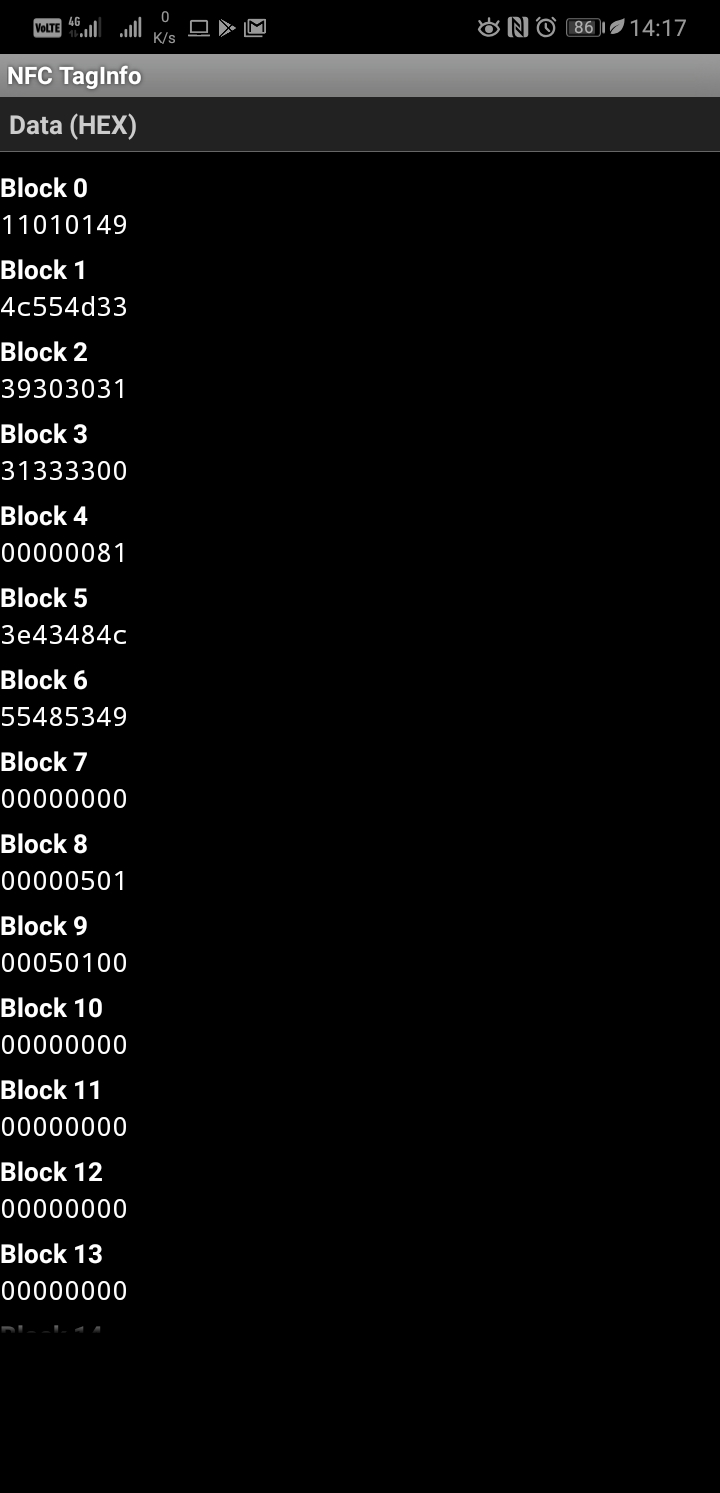
\includegraphics[keepaspectratio,width=\linewidth]{RFID_Blocks-Hex}
		\caption{Blöcke in Hex mit Smarphone ausgelesen}
	\end{subfigure}
	\begin{subfigure}[t]{.45\textwidth}
		\centering
		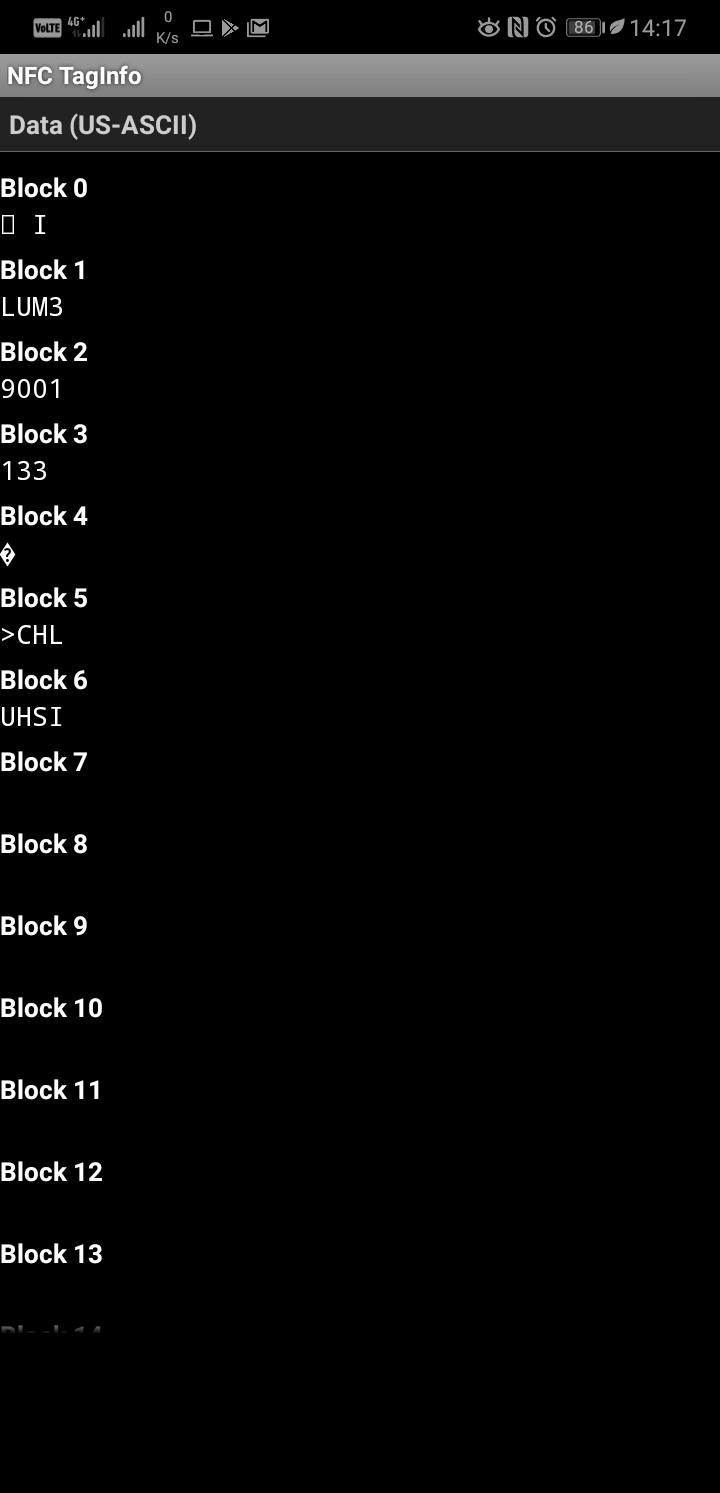
\includegraphics[keepaspectratio,width=\linewidth]{RFID_Blocks-Ascii}
		\caption{Blöcke in ASCII mit Smarphone ausgelesen}
	\end{subfigure}
	\begin{subfigure}[b]{.3\textwidth}
		\centering
		
\includegraphics[keepaspectratio,width=\linewidth]{Barcode_BuchRFIDTag}
		\caption{Zugehöriger Barcode}
	\end{subfigure}
	\caption{Ausgelesene Blöcke und Barcode des Buches}
	\label{fig:AusgeleseneBloeckeUndBarcode}
\end{figure}


\clearpage
\section{Systemspezifikation Referenzimplementation}
\label{sec:SysSpec}

\subsection{Anforderungen}
\label{sub:ReferenzimplementationAnforderungen}
Hier werden die Anforderungen an die Referenzimplementation, welche bereits in Kapitel \ref{sub:Anforderungen} erwähnt wurden, nochmals aufgelistet.
\begin{legal}
	\item Die Referenzimplementation ist in der Lage die Buch ID eines Exemplares über RFID auszulesen.
	\item Die Referenzimplementation soll erkennen, wenn eine Box ein Exemplar (eines, welches mit RFID ausgestattet ist und technisch auch Lesbar ist) enthält, welches nicht dieser Box zugehörig ist.
	\item Die Referenzimplementation soll jede erkannte Unstimmigkeit (Exemplar, welches nicht zu diesem Behälter gehört) in einem Logdokument persistieren.
	\item Die Referenzimplementation soll in der Lage sein, dem Endbenutzer, in graphischer Form durch eine Konsolen-Ausgabe, mitzuteilen, welcher Behälter eine Unstimmigkeit enthält.
	\item Die Referenzimplementation soll die unter Laborbedingungen erhaltenen Resultate unter Realbedingungen verifizieren.
	\item Die Referenzimplementation soll mit einer Oracle Datenbank kommunizieren können.
\end{legal}

\subsection{Kontext}

Das nachfolgende Kontextdiagramm (Abbildung \ref{fig:Kontextdiagramm}) beschreibt die Interaktion der Referenzimplementation mit allen Umsystemen. Diese Umsysteme beinhalten den Benutzer, welche von der Referenzimplementation Informationen erhält, ein weiteres Umsystem beinhaltet ein Datenbankexport Dokument, welches dem System die Informationen zu einem Exemplar liefert. Das Letzte Umsystem ist die der RFID Reader, welches dar Referenzimplementation die Informationen eines gefundenen RFID Tags liefert.
\begin{figure}[htb]
	\centering
	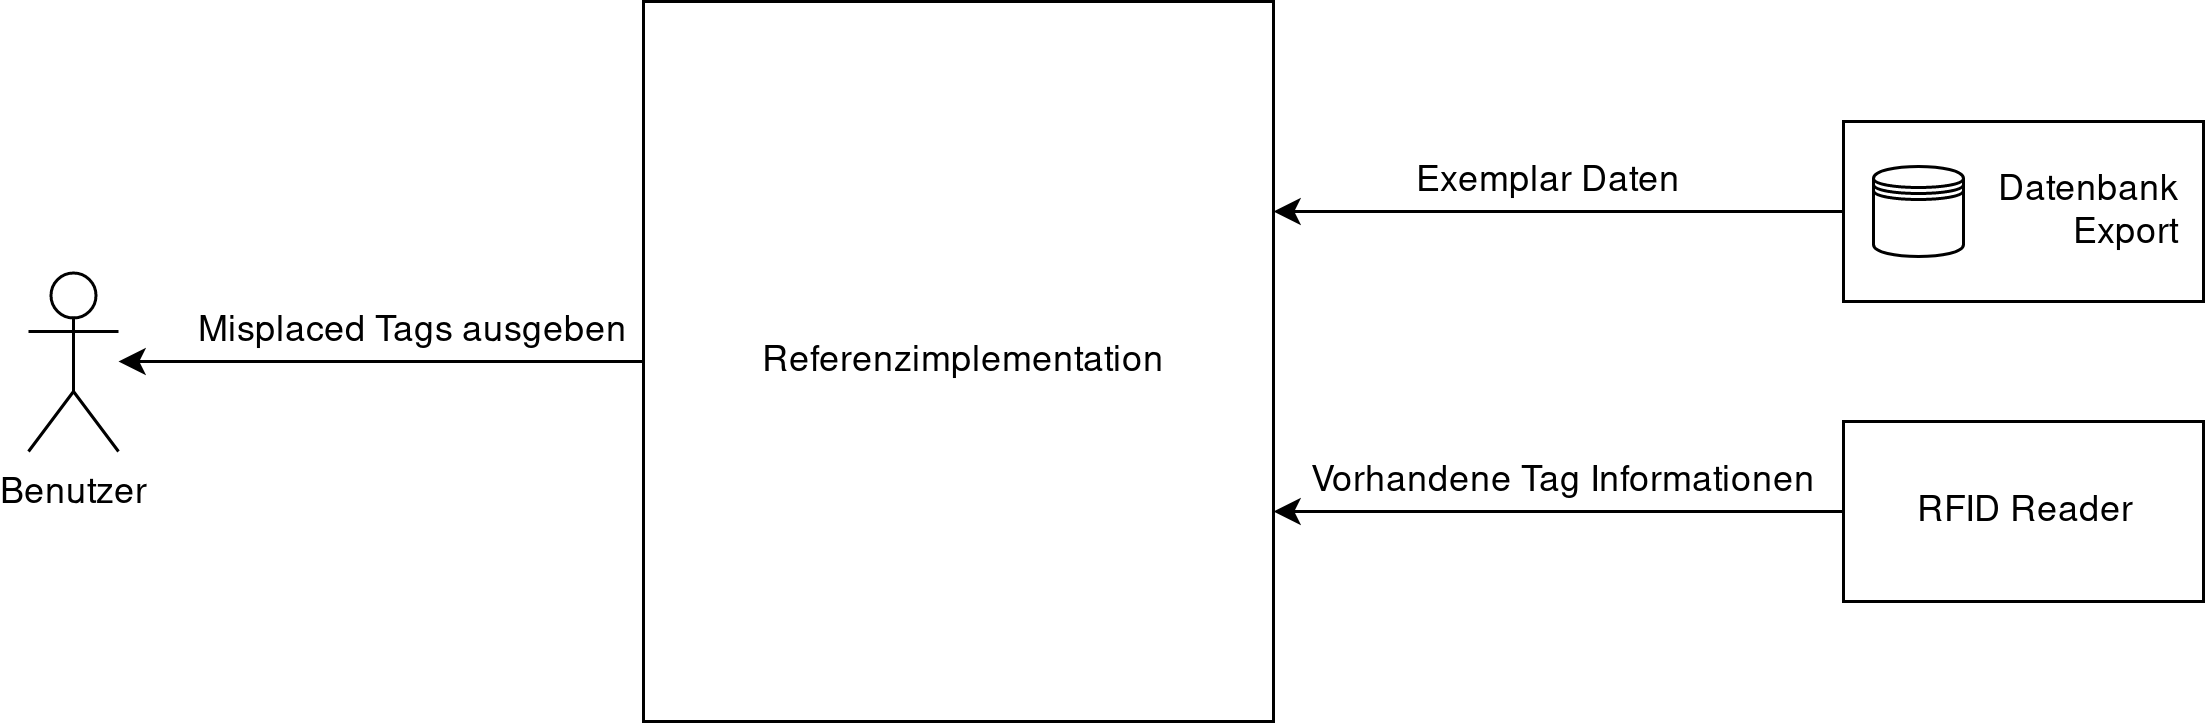
\includegraphics[keepaspectratio,width=.9\linewidth]{Kontextdiagramm}
	\caption{Kontextdiagramm der Referenzimplementation}
	\label{fig:Kontextdiagramm}
\end{figure}

\subsection{System}

\subsection{Komponenten}


\subsection{Interne Schnittstellen}

\subsection{Klassendiagramm}

\subsection{Anforderungen der Software}

\subsection{Umsetzung Programmierung}

\subsection{Testing}


\section{Projektorganisation}

\vspace{1em}

\begin{tabularx}{\textwidth}{|X|X|}
	\hline
	\textbf{Projektbeteiligte} & \textbf{Funktionen} \\
	\hline
	Mike Märki & Stakeholder/Auftraggeber \\
	\hline
	Martin Jud & BDA Experte \\
	\hline
	Pascal Baumann & Product Owner \& Dev Team \\
	\hline
	Dane Wicki & Scrum Master \& Dev Team \\
	\hline
\end{tabularx}

\subsection{Organigramm}
\begin{figure}[h!]
	\centering
	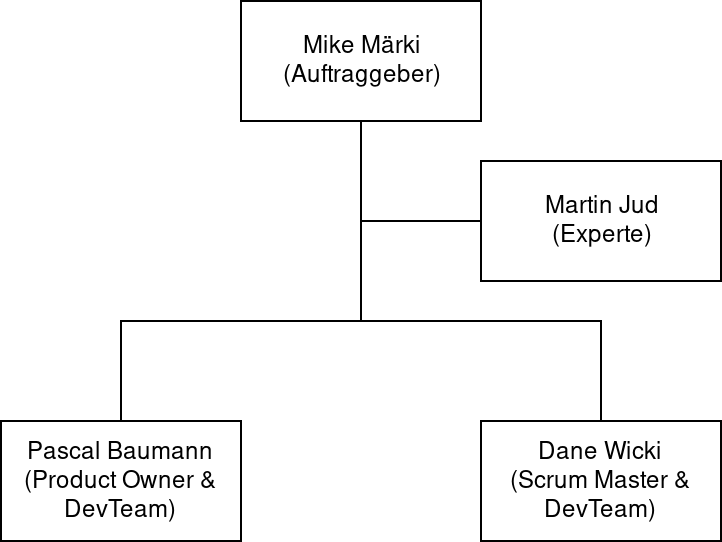
\includegraphics[keepaspectratio, width=0.6\textwidth]{OrganigrammBDA_BAWI.png}
\end{figure}

\subsection{Rollen im Team}
Hier werden die Hauptverantwortlichkeiten des Jeweiligen Teammitgliedes niedergeschrieben. Dies bedeutet nicht, dass dieses jeweilige Mitglied für diese Funktion, Tätigkeit oder Aufgabe alleine zuständig war, sondern lediglich, dass die Entscheidungsgewalt, sowie die Verantwortung bei diesem liegt.

\begin{tabularx}{\textwidth}{|l|X|}
	\hline
	\textbf{Teammitglied} & \textbf{Funktion/Tätigkeit/Aufgaben} \\
	\hline
	Pascal Baumann & Stand der Forschung \\
		& Konzept 2 (Verhinderung des Deplatzieren eines Exemplars) \\
		& Machbarkeitstudie Recherche \\
		& Support Dokumentationssoftware \\
		& Grobplanung \\
		& Risikoanalyse \\
		& CI/CD Dokumentation \\
	\hline
	Dane Wicki & Konzept 1 (Auffindung eines deplatzierten Exemplars)\\
		& Requirements Engineering \\
		& Softwarearchitektur \\
		& Programming Language Advisor \\
		& CI/CD Software \\
		& RFID Hardwarebeschaffung und Verwaltung \\
		& Hardware Interface Specialist \\
		& Sitzungsprotokolle \\
		
	\hline
\end{tabularx}

\section{Rahmenplan}
\subsection{Meilensteine}
\label{ssec:Meilensteine}
Für das Projekt wurden vier Meilensteine definiert, welche jeweils im Vierwochenzyklus auftreten. Diese Meilensteine sind in Abbildung \ref{fig:Milestones} dargestellt.

\begin{figure}[h!]
	\centering
	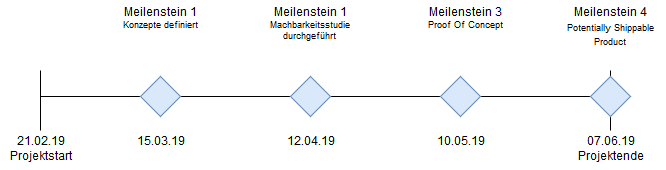
\includegraphics[keepaspectratio,width=0.8\linewidth]{Milestones.png}
	\caption{Die für das Projekt definierten Meilensteine}
	\label{fig:Milestones}
\end{figure}

\subsection{Grobplan}

Aus den im Kapitel \ref{ssec:Meilensteine} definierten Meilensteine wurden acht Sprints von zwei Wochen abgeleitet. In diesen werden sowohl die Artefakte wie Projektdokumentation, Machbarkeitsstudien und Systemspezifikation, wie auch das Produkt entwickelt. Der grobe Rahmenplan ist in Abbildung \ref{fig:Rahmenplan_1} dargestellt.

\begin{figure}[h!]
	\centering
	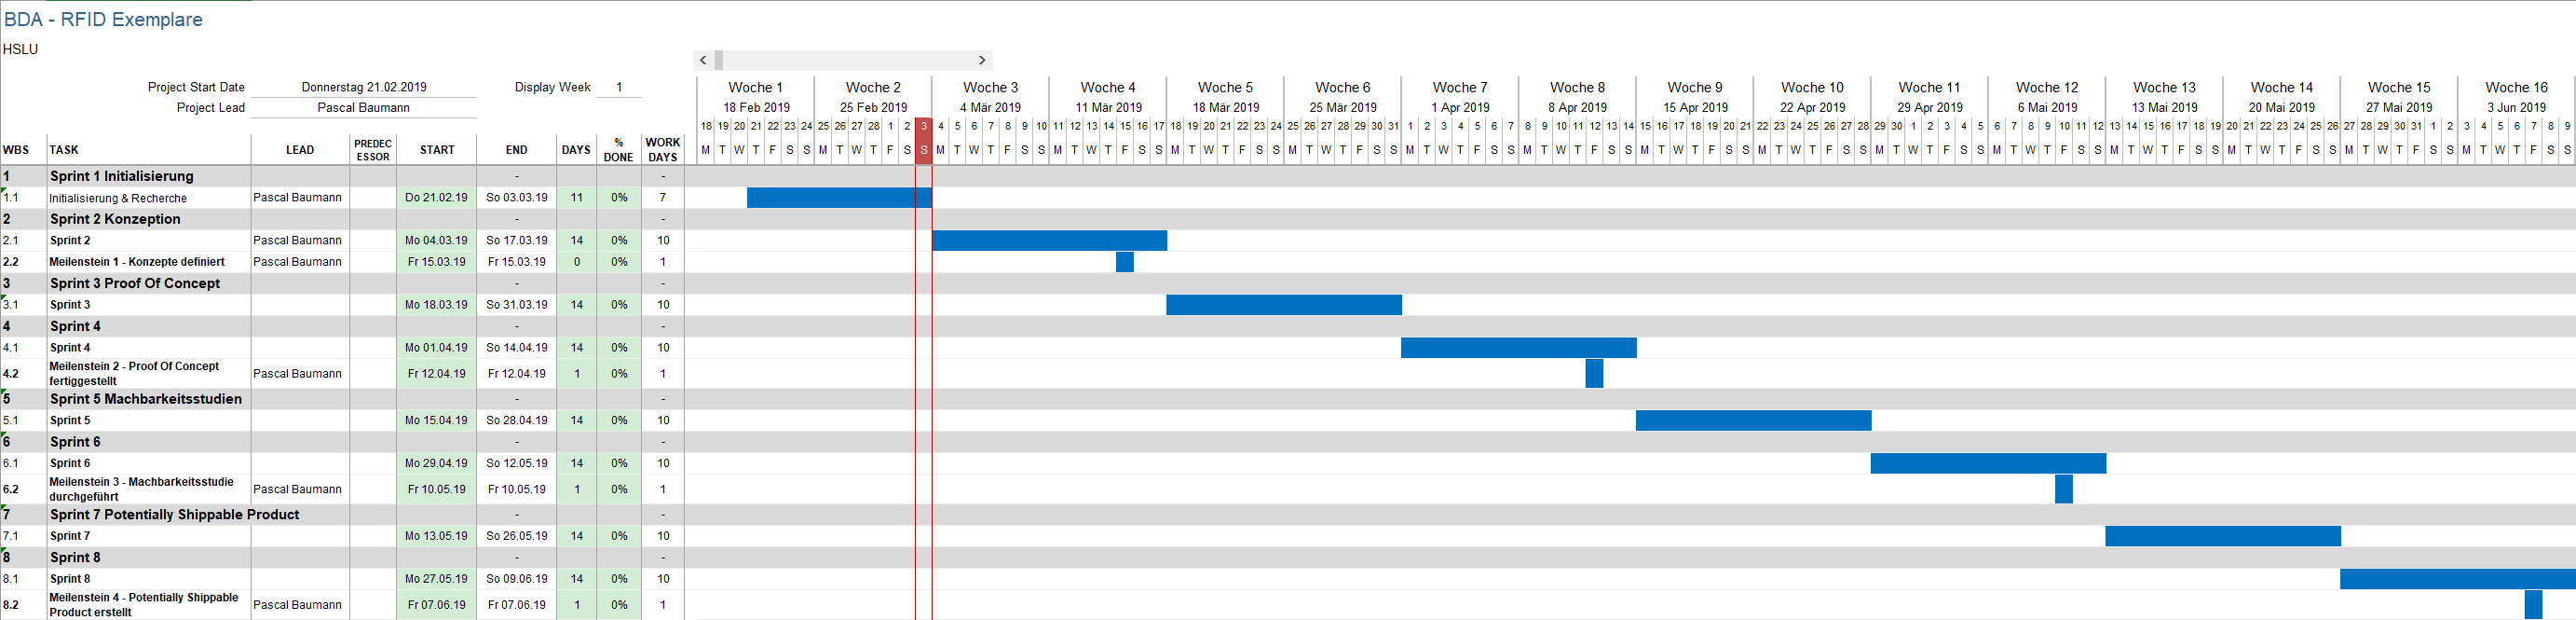
\includegraphics[keepaspectratio,width=\linewidth]{Grobplan.png}
	\caption{Übersicht der Sprints im Rahmenplan}
	\label{fig:Rahmenplan_1}
\end{figure}

\section{Beschreibung der Sprints}

\subsection{Sprint 01}
Das Sprintziel des ersten Sprints war der Wissensaufbau bezüglich RFID und wie eine Machbarkeitsstudie durchgeführt werden muss.

Im Vorfeld erstellte Herr Baumann einen Grobplan, eine erste Risikoanalyse und bereitete die Struktur der Dokumentation vor. Das Team bereitete sich auf das Meeting vor, indem es sich intensiv mit der Aufgabenstellung auseinandersetzte und bereits technische Überlegungen anstellte. Ungewissheiten wurden dabei gleich als Fragen für den Kunden erarbeitet, zudem wurde ein grober Zeitplan erarbeiteten. Das Kickoff-Meeting wurde aufgezeichnet und von Herrn Wicki in ein Protokoll transkribiert. Danach begann Herr Wicki mit der Anforderungsanalyse und Aktualisierte die Aufgabenstellung mit den gewonnenen Erkenntnissen. Herr Baumann las sich in die Erstellung einer Machbarkeitsstudie ein und erarbeitete ein Merkblatt für das Team. Das Projektteam las sich in die RFID Protokolle ein und erstellte einen ersten Entwurf der Stand der Technik, Herr Baumann konzentrierte sich dabei mehr um die technischen und theoretischen Voraussetzungen, während Herr Wicki über Referenzimplementationen Recherchen anstellte. Unter anderem wurde dabei der Hersteller der aktuell in der Speicherbibliothek eingesetzten Geräte ermittelt. Insgesamt verlief dieser Sprint aufgrund der Vorbereitungsarbeiten sehr flüssig und gab dem Projekt von Anfang an einen Aufwind.

Angetroffene Probleme waren die Unbekannten im Bezug auf das Projekt und wie eine Machbarkeitsstudie durchgeführt werden soll. Durch die Planung konnten diese Probleme jedoch angegangen werden. Es wurde ein Merkblatt zur Durchführung einer Machbarkeitsstudie erstellt und dem Team präsentiert und durch die Recherchen konnten technische Limitationen von HF RFID identifiziert werden.

\subsection{Sprint 02}
Das Sprintziel des zweiten Sprints waren die Erarbeitung und Spezifikation von zwei Konzepten.

Daher wurden die Erkenntnisse aus der Recherchephase umgesetzt. Im Speziellen erhielt Herr Baumann den Auftrag eine Struktur für die Machbarkeitsstudie zu erarbeiten und dem Team zur Verfügung zu stellen, er sollte auch die bestehende Projektdokumentation den Vorgaben der Hochschule für studentische Arbeiten anpassen. Nach einer Ideenfindung einigte man sich im Team zwei Konzeptideen genauer auszuarbeiten. Herr Baumann konzentrierte sich dabei auf eine stationäre Lösung beim Rüstplatz, während Herr Wicki ein Konzept für die automatische Suche im Lager erarbeitete. Beide Lösungskonzepte wurden anschliessend im Team präsentiert. Daraus ergab sich die Notwendigkeit Hersteller anzufragen, welche Lösungen mit einer Reichweite von mindesten 90cm anbieten. Herr Wicki fasste diesen Auftrag und ermittelte zwei passende, in Europa ansässige Hersteller. Die zwei erarbeiteten Konzepte wurden in einer Sitzung dem Kunden präsentiert und abgenommen. Insgesamt verlief dieser Sprint gut und es konnten Fortschritte in alle Richtungen (Projekt, Dokumentation, Kundendeliverables) verzeichnet werden.

Probleme verursachten vor allem die Ideenfindung für die Konzepte, insbesondere die Idee einer Suchbox stellte sich als schwierig an, da die Recherchen ergaben, dass die maximale Lesereichweite von HF RFID Lesern bei knapp einem Meter lag. Das Problem wurde durch eine gemeinsame Ideenfindung und Ausarbeitung der Konzeptidee gelöst. Danach wurden die Konzepte erfolgreich spezifiziert, dokumentiert und ausgearbeitet. Das Sprintziel konnte somit erfolgreich erreicht werden und die interne Zusammenarbeit verlief effizient und sehr zufriedenstellend.

\subsection{Sprint 03}
Das Sprintziel des dritten Sprints war die Akquisition und insbesondere Erhalt, eines HF RFID-Lesegeräts mit mindestens zwei Antennen.

Aus der Meilensteinsitzung wurde klar, dass die Kosten für die ermittelten Geräte für Testzwecke und Prototypisierung zu hoch sind, und die nötigen Geldmittel weder vom Kunden noch vonseiten der Hochschule zur Verfügung stehen. Als Sprintziel wurde die Akquisition von Versuchsgeräten definiert. Das Projektteam versuchte noch einmal Testgeräte bei Bildungseinrichtungen, Hochschulen und Herstellern zu erhalten. Herr Baumann kontaktierte dafür Gewerbeschulen in der Zentralschweiz und Kompetenzzentren für RFID an den Hochschulen Luzern und Winterthur. Herr Wicki kontaktierte Vertreiber von HF RFID Lösungen, ob diese Leihgeräte zur Verfügung stellen könnten. Weiter wurden auch die Budgetvorstellungen der Hochschule dem Projektteam mitgeteilt. Weiter wurde vom Projektteam das Protokoll für die Meilensteinsitzung erarbeitet. Die Herausforderung in diesem Sprint waren vor allem die Schwierigkeiten im Bezug auf die Versuchsgeräte, insbesondere der Erhalt der Vielzahl von Absagen.

In diesem Sprint stellten sich vor allem Budgetprobleme vonseiten des Kunden und der Hochschule. Gelöst werden konnte diese nur durch Eigeninvestitionen und günstigeren Produkten aus China. Da die Produkte nur bestellt, aber nicht bei uns eingetroffen waren, konnte das Sprintziel nicht erreicht werden. Positiv war, dass durch die agile Projektmethode auf das Problem reagiert werden konnte, und dieser und subsequente Sprints umgeplant werden konnte.

\subsection{Sprint 04}
Das Sprintziel des vierten Sprints war die Fertigstellung, das heisst Implementation aller kritischen Komponenten, sodass die Versuche durchgeführt werden konnten, des Testframeworks bis auf Treiber und die Definition der Versuche.

In diesem Sprint wurden die erarbeiteten Konzepte noch einmal kritisch begutachtet, harmonisiert und für die Machbarkeitsstudie finalisiert. Alle Versuche Leihgaben zu erhalten scheiterten jedoch. Vonseiten der Hersteller erhielt man zwar Rabatte. Die Preise für die Geräte waren jedoch immer noch ein Vielfaches von dem, was die Hochschule bereit war für eine BDA zur Verfügung zu stellen. Das Team entschied sich, um reelle Aussagen in der Machbarkeitsstudie machen zu können, auf eigene Kosten bei einem Hersteller in China zu bestellen. Diese Geräte trafen dann auf Ende Sprint beim Team ein. Um nicht zu viel Zeit zu verlieren, entschied das Team sich, Versuche genau zu spezifizieren, Versuchsmaterialien zu beschaffen und ein Testframework zu definieren. Dieses war vor allem nötig um im Millisekundenbereich Gerätefunktionen zu testen, was von Hand gar nicht oder nur begrenzt möglich ist. Am Ende dieses Sprints stand die Zwischenpräsentation des Projekts an. Diese wurde von beiden Teammitgliedern erarbeitet, antrainiert und dem Betreuer und Experten präsentiert. Die Herausforderung dieses Sprints war der Motivationsdämpfer aufgrund der Schwierigkeiten und Ungewissheit im Bezug auf die Versuchsgeräte und dem weiteren Verlauf des Projekts.

Der Sprint war durch eine Vielzahl von Problemen geplagt. Zum einen war dies die späte Ankunft der Testgeräte auf das Ende des Sprints, zum zweiten die Verzögerung des Abschlusses des letzten Sprints und dadurch eine Verkürzung dieses Sprints und zum Schluss fehlende Ressourcen durch die Arbeitstätigkeit eines Teammitglieds. All dies führte dazu, dass das Sprintziel nicht erreicht wurde. Um einen solchen Sprint nicht noch einmal erleben zu müssen, wurde am Anfang des nächsten Sprints eine detaillierte Retrospektive durchgeführt und Massnahmen definiert. Das Resultat war eine klar fixierte Zeit für ein wöchentlich stattfindendes, telefonisches Meeting und Austausch zwischen den Teammitgliedern.

\subsection{Sprint 05}
Das Ziel des fünften Sprints war die Durchführung und Dokumentation der im letzten Sprint definierten Versuche.

Bevor die Versuche durchgeführt werden konnten, musste ein Treiber für die Geräte entwickelt werden. Herr Wicki fragte diesbezüglich beim Händler die Spezifikation der Schnittstelle an und entwickelte einen Treiber. Herr Baumann kümmerte sich um die Benutzerschnittstelle und das Einpflegen der Versuchsdefinitionen. Weiter begann die Arbeit an der Machbarkeitsstudie, wobei Herr Baumann das Projektumfeld der Machbarkeitsstudie und Herr Wicki die Beschreibung des Projektes im Kontext der Machbarkeitsstudie in Angriff nahm.

Das angetroffene Problem dieses Sprints war, dass die Spezifikation des Gerätetreibers weniger gut als erhofft war. Insbesondere muss die DLL des Händlers verwendet werden, welche nur durch eine 32bit Applikation aufgerufen werden kann, und dazu keine Betriebssystemunabhängigkeit zulässt. Gelöst wurde dies, indem Windows und JNI/JNA verwendet wurde. Positiv war, dass das Sprintziel erfolgreich erreicht und die angetroffenen Probleme behoben werden konnten.

\subsection{Sprint 06}
Das Sprintziel dieses Sprints lag in der Fertigstellung der Machbarkeitsstudie.

Bedingt durch das Sprintziel wurden die Kapitel der Machbarkeitsstudie in jeweils 5-13h Arbeitspakete unterteilt und diese anschliessend unter beiden projektdurchführenden Personen aufgeteilt. So schrieb Herr Wicki die Kapitel Investitions- und Betriebskosten, Beschreibung des Projekts, technische Aspekte und das Finding Summary wie auch das Abstract. Herr Baumann schrieb seinerseits die Kapitel Projektumfeld, Entwicklungsplan und markttechnische Aspekte.
Gegen Ende des Sprints gab es zudem noch eine Meilensteinsitzung, bei welcher die erarbeiteten Artefakte, namentlich die Machbarkeitsstudie wie auch die Ergebnisse der Tests, an Herr Märki präsentiert und abgegeben wurde. Bei dieser Meilensteinsitzung wurden noch die Anforderungen für die kommende Entwicklung des MVPs besprochen, da einige Anforderungen noch zu generisch beschrieben waren. Bei dieser Absprache konnte schliesslich noch ein Missverständnis identifiziert werden, bei welchem das Team davon ausging, dass die Tag-ID in der Datenbank gespeichert ist, jedoch sei nicht der Fall ist und nur die Buch-ID, welche auch als Barcode auf dem Buch ist, in der Datenbank zu finden ist. Anschliessend wurden alle Anforderungen nochmals durchgegangen und auf deren Erfüllung überprüft.

Die Probleme während diesem Sprint hielten sich in Grenzen. So gab es lediglich das Problem, dass keiner der beiden Studierenden mit dem Schreiben einer Machbarkeitsstudie stark vertraut war und es dadurch zu der Situation kam, bei welcher eine Tabelle dupliziert im Dokument anzutreffen war. In einer kurzen Besprechung konnte jedoch gemeinsam der passende Absatz im Dokument gefunden werden für diese Tabelle, sodass diese nur noch einmal vorhanden ist.

\newpage

\section{Tools}
\label{sec:Tools}

\subsection{Versions Kontrolle}
\begin{table}[h!]
	\begin{tabular}{p{0.5\textwidth} p{0.5\textwidth}}
		\hline
		\textbf{Tool} & \textbf{Version} \\
		\hline
		GitKraken & 4.2.2 \\
		\hline
		git & 2.21.0 \\
		\hline
		GitHub & GitHub.com \\
		\hline
	\end{tabular}
	\caption{Verwendete Versionen der Versionierungssysteme}
\end{table}

\subsection{Dokumentation}
\begin{table}[h!]
	\begin{tabular}{p{0.5\textwidth} p{0.5\textwidth}}
		\hline
		\textbf{Tool} & \textbf{Version} \\
		\hline
		TeX Live & 2018 \\
		\hline
		MiKTex & 2.9.6637 \\
		\hline
		Mendeley Desktop & 1.19.2 \\
		\hline
		MS Excel & 16.0.11231.20164 \\
		\hline
	\end{tabular}
	\caption{Verwendete Versionen der Hilfsmittel für die Dokumentation}
\end{table}


\subsection{Repositories \& Buildtools}
\begin{table}[h!]
	\begin{tabular}{p{0.5\textwidth} p{0.5\textwidth}}
		\hline
		\textbf{Name} & \textbf{URL} \\
		\hline
		Dokumentation & \url{https://github.com/HSLU-BaumannWicki/BDA_FS19-Dokumentation} \\
		\hline	
		Travis CI &  \url{https://travis-ci.org/HSLU-BaumannWicki/BDA_FS19-Dokumentation} \\
		\hline
	\end{tabular}
	\caption{Verwendete Repositories}
\end{table}

\subsection{Übrige}
\begin{table}[h!]
	\begin{tabular}{p{0.5\textwidth} p{0.5\textwidth}}
		\hline
		\textbf{Tool} & \textbf{Verwendung} \\
		\hline
		Trello & Aufgabenverwaltung \\
		\hline
		Scrum Poker Online & Storypoints Estimation\\
		\hline
		WhatsApp & Kommunikation im Team \\
		\hline
		OneDrive Online & Dokumentenspeicher \\
		\hline	
	\end{tabular}
	\caption{Übrige Hilfsmittel}
\end{table}

\clearpage

\section{Risikomanagement}

Es werden mögliche Risiken, welche während dem Projekt auftreten können aufgezählt. Diese werden auf Eintrittswahrscheinlichkeit und Schadensmass eingeschätzt, danach wird entschieden, welche Massnahmen getroffen werden können, und was deren Auswirkungen sind.

\subsection{Definitionen}
\label{sssec:Def}
\vspace{1em}
\noindent
Eintrittswahrscheinlichkeit:

\vspace{1em}
\noindent
\begin{tabularx}{\textwidth}{|l|l|X|}
	\hline
	\textbf{Stufe} & \textbf{Bezeichnung} & \textbf{Beschreibung} \\
	\hline
	1 & unvorstellbar & Möglich aber eher unwahrscheinlich. Tritt nie oder einmal in 16 Wochen auf \\
	\hline
	2 & unwahrscheinlich & Kann in 16 Wochen kein oder ein Mal eintreten\\
	\hline
	3 & vorstellbar & Kann in 16 Wochen ein bis zwei Mal eintreten \\
	\hline
	4 & wahrscheinlich & Kann in 16 Wochen bis zu drei Mal eintreten \\
	\hline
	5 & häufig & Kann in 16 Wochen sieben Mal eintreten\\
	\hline
\end{tabularx}

\vspace{1em}
\noindent
Schadensausmass:

\vspace{1em}
\noindent
\begin{tabularx}{\textwidth}{|l|l|X|}
	\hline
	\textbf{Stufe} & \textbf{Bezeichnung} & \textbf{Beschreibung} \\
	\hline
	1 & unwesentlich & Die Aufgabenerfüllung wird höchstens geringfügig beeinträchtigt, finanzieller Schaden ist im Rahmen des Projekts nicht beeinflussend. Personenschäden treten nicht auf. \\
	\hline
	2 & geringfügig & Wahrnehmbare Gefährdung / Einfluss auf das Projekt. Personenschäden treten nicht auf. \\
	\hline
	3 & mittelmässig & Wahrnehmbare Gefährdung / Einfluss auf das Projekt. Verzögerungen zur Folge. Finanzieller Schaden strapaziert das Projektbudget. Personenschäden treten nicht auf. \\
	\hline
	4 & kritisch & Starke Gefährdung des Projekts. Extreme Verzögerungen zur Folge. Finanzieller Schaden übersteigt das Projektbudget. Personenschäden treten geringfügig auf.\\
	\hline
	5 & katastrophal & Projektabbruch zur Folge. Finanzieller Schaden kann zum Projektstopp führen. Verletzung der Persönlichkeitsrechte. \\
	\hline
\end{tabularx}

\newpage

\subsection{Risikokatalog}
\label{sssec:Risikokatalog}
Legende:
\begin{itemize}
	\item \textbf{S}chadensausmass bei Eintreffen des Risikos
	\item \textbf{W}ahrscheinlichkeit das Risiko eintrifft
	\item \textbf{K}ategorie: \textbf{T}echnisches oder \textbf{P}rojektbezogenes Risiko
	\item \textbf{A}uswirkung auf das Projekt. Produkt aus S und W
\end{itemize}

\vspace{1em}
\noindent
\begin{table}[htb]
	\begin{tabularx}{\textwidth}{|l|X|l|l|l||l|}
		\hline
		\textbf{Nr.} & \textbf{Beschreibung / Risiko} & \textbf{K} & \textbf{S} & \textbf{W} & \textbf{A} \\
		\hline
		1 & Meilensteine werden nicht erreicht & P & 4 & 2 & 8 \\
		\hline
		2 & Teammitglied fällt aus & P & 4 & 1 & 4 \\
		\hline
		3 & Fehlkommunikation im Team & P & 4 & 1 & 4 \\
		\hline
		4 & Produkt entspricht nicht den Kundenanforderungen & P & 5 & 2 & 10 \\
		\hline
		5 & Umsetzung des Produkts technisch nicht möglich & T & 3 & 3 & 9 \\
		\hline
		6 & Datenverlust & T & 5 & 2 & 10 \\
		\hline
		7 & Lieferschwierigkeiten von Teilen & P & 3 & 3 & 9 \\
		\hline
		8 & Kosten übersteigen Budgetvorstellung des Kunden & P & 3 & 2 & 6\\
		\hline
		9 & Kosten übersteigen Budgetvorstellung der Hochschule & P & 3 & 3 & 9\\
		\hline
	\end{tabularx}
	\caption{Die im Projekt identifizierten Risiken}
	\label{tbl:Risks}
\end{table}

\vspace{1em}

\begin{figure}[h!]
	\centering
	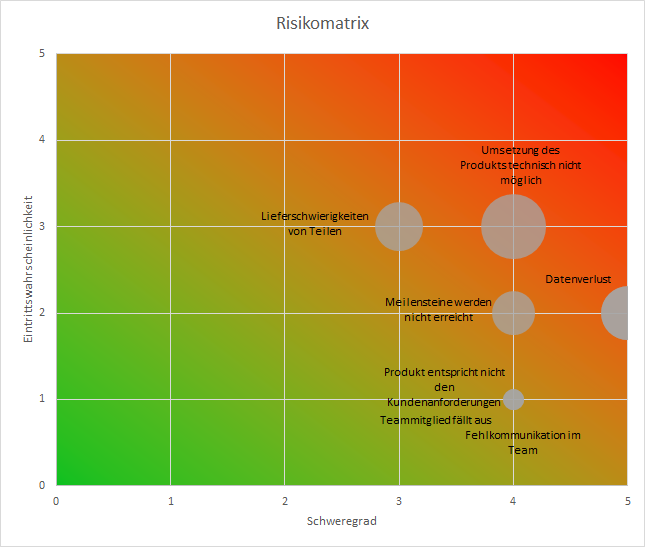
\includegraphics[keepaspectratio, width=0.6\textwidth]{Risks_before.png}
	\caption{Auswirkungen der in Tabelle \ref{tbl:Risks} identifizierten Risiken}
\end{figure}

\newpage

\subsubsection{Massnahmen}

\begin{table}[htb]
	\begin{tabularx}{\textwidth}{|l|X|}
		\hline
		\textbf{Nr.} & \textbf{Beschreibung Massnahme} \\
		\hline
		1 & Meilensteine werden in zwei Zweiwöchigen Sprints absolviert. Die Tasks pro Sprint werden weiter detailliert heruntergebrochen. So sollen die Arbeiten sowohl auf Makro- wie Mikrosicht eingeplant werden. \\
		\hline
		2 & Arbeiten werden so strukturiert und dokumentiert, dass das zweite Mitglied diese auch übernehmen kann. Es werden Spezialisierungen der Teammitglieder insoweit verhindert, dass Wissenslücken minimiert werden. Recherchen sollen Zusammenfassungen und Merkblätter über die gewonnenen Erkenntnisse als Resultat haben.\\
		\hline
		3 & Der Kontakt wird von beiden Teammitgliedern sowohl horizontal im Team wie auch vertikal zu den Stakeholdern aktiv gesucht. Es werden den Arbeiten auch teambildende Aktivitäten zusammen absolviert.\\
		\hline
		4 & Der Kunde muss den Fortschritt alle vier Wochen in einer Sitzung kontrollieren, avisieren und, wenn nötig, Anpassungen fordern.\\
		\hline
		5 & Es soll während den Recherchen schon im Hinblick auf die technische Umsetzung acht gegeben werden.\\
		\hline
		6 & Sowohl produzierten Artefakte, wie auch aktuelle getätigte Arbeiten werden auf auswärtige Plattformen ausgelagert.\\
		\hline
		7 & Teile werden bei Bedarf sofort bestellt, es werden inländische, etablierte Lieferanten, vor evtl. günstigeren Ausländischen vorgezogen.\\
		\hline
		8 & Lösungskonzept wird in der erarbeiteten Form verworfen und durch günstigere Komponenten ersetzt.\\
		\hline
		9 & Es werden alternative Sponsoren von Geldmittel gesucht.\\
		\hline
	\end{tabularx}
	\caption{Massnahmen um Effekte oder Eintrittswahrscheinlichkeit zu reduzieren}
\end{table}

\vspace{1em}

\begin{table}[htb]
	\begin{tabularx}{\textwidth}{|l|X|l|l|l||l|}
		\hline
		\textbf{Nr.} & \textbf{Beschreibung / Risiko} & \textbf{K} & \textbf{S} & \textbf{W} & \textbf{A} \\
		\hline
		1 & Meilensteine werden nicht erreicht & P & 4 & 1 & 4 \\
		\hline
		2 & Teammitglied fällt aus & P & 3 & 1 & 3 \\
		\hline
		3 & Fehlkommunikation im Team & P & 4 & 1 & 4 \\
		\hline
		4 & Produkt entspricht nicht den Kundenanforderungen & P & 5 & 1 & 5 \\
		\hline
		5 & Umsetzung des Produkts technisch nicht möglich & T & 4 & 3 & 12 \\
		\hline
		6 & Datenverlust & T & 5 & 1 & 5 \\
		\hline
		7 & Lieferschwierigkeiten von Teilen & P & 3 & 2 & 6 \\
		\hline
		8 & Kosten übersteigen Budgetvorstellung des Kunden & P & 3 & 1 & 3\\
		\hline
		9 & Kosten übersteigen Budgetvorstellung der Hochschule & P & 3 & 2 & 6\\
		\hline
	\end{tabularx}
	\caption{Neueinschätzung der Risiken nach Einführung der Massnahmen}
	\label{tbl:Massnahmen}
\end{table}

\vspace{1em}

\begin{figure}[h!]
	\centering
	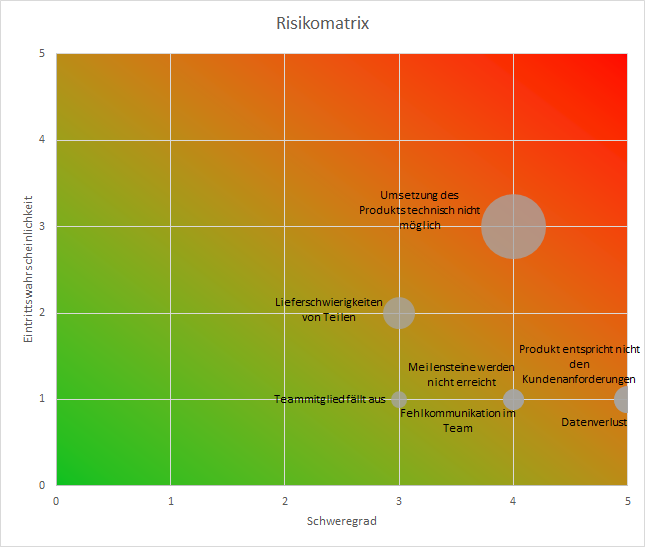
\includegraphics[keepaspectratio, width=0.6\textwidth]{Risks_after.png}
	\caption{Auswirkungen der Risiken nach den in Tabelle \ref{tbl:Massnahmen} vorgeschlagenen Massnahmen}
\end{figure}


\chapter{Evaluation und Validation}
\label{ch:Eval}
In diesem Kapitel wird evaluiert, ob das Projekt und dessen produzierte Artefakte die Anforderungen erfüllen. Dazu wurden alle Anforderungen nochmals zusammengetragen und jede einzelne mit dem jeweiligen Artefakt überprüft, das Resultat wurde schliesslich in Form einer einfach lesbaren Tabelle festgehalten. Aus dem Vergleich der konnte schliesslich festgestellt werden, dass alle priorisierten Anforderungen erfüllt werden konnten. Daher kann dieses Projekt als erfolgreich betrachtet werden.

\section{Vergleich mit Anforderungen}
\label{sec:VergleichAnforderungen}
Hier werden die Anforderungen aufgelistet und ob diese erfüllt wurden oder nicht. Sofern diese nicht erfüllt wurden, wird für deren Erfüllung eine potenzielle Lösungsidee beschrieben. Für die Verifikation wurden die Testfälle überprüft.

Legende:
<<\checkmark >> = Anforderung erfüllt, <<\xmark>> = Anforderung nicht erfüllt, <<->> Wurde aus den beschriebenen Gründen nicht Implementiert.


\begin{tabularx}{\textwidth}{l l X}
	\hline
	\checkmark & 1   & Es sollen mindestens zwei Lösungskonzepte für eine als Auswahl der Machbarkeitsstudie entwickelt werden. \\
	\hline
	\checkmark & 2   & Die Lösungskonzepte müssen auf deren technische Realisierbarkeit untersucht werden. \\
	\hline
	\checkmark & 3   & Es muss mindestens ein entwickeltes Konzept für die Machbarkeitsstudie verwendet werden. \\
	\hline
	\checkmark & 4   & Die Machbarkeitsstudie muss eine Kostenrechnung für die Lösungsansätze beinhalten. \\
	\hline
	\checkmark & 5   & Es soll eine Referenzimplementation entwickelt werden, welche vom Kunde verwendet werden kann. \\
	\hline
	\checkmark & 6.1 & Die Lösungskonzepte müssen mit dem Lagersystem kommunizieren können \\
	\hline
	\checkmark & 6.2 & Die Lösungskonzepte müssen die RFID Tags in weniger als 1 Sekunden identifizieren können. \\
	\hline
	\checkmark & 6.3 & Die Lösungskonzepte müssen für das bestehende Hochregallager der Speicherbibliothek verwendbar sein. \\
	\hline
	\checkmark & 7.1 & Das Proof of Concept muss technisch aufzeigen, wie viele RFID Tags in einer Sekunde identifiziert werden können. \\
	\hline
	\checkmark & 8.1 & Die Referenzimplementation ist in der Lage die Buch ID eines Exemplares über RFID auszulesen. \\
	\hline
	\checkmark & 8.2 & Die Referenzimplementation soll erkennen, wenn eine Box ein Exemplar (eines, welches mit RFID ausgestattet ist und technisch auch Lesbar ist) enthält, welches nicht dieser Box zugehörig ist. \\
	\hline
	\checkmark & 8.3 & Die Referenzimplementation soll jede erkannte Unstimmigkeit (Exemplar, welches nicht zu diesem Behälter gehört) in einem Logdokument persistieren. \\
	\hline
	\checkmark & 8.4 & Die Referenzimplementation soll in der Lage sein, dem Endbenutzer, in graphischer Form, durch eine Konsolen-Ausgabe, mitzuteilen, welcher Behälter eine Unstimmigkeit enthält. \\
	\hline
	? & 8.5 & Die Referenzimplementation soll die unter Laborbedingungen erhaltenen Resultate unter Realbedingungen verifizieren. \\
	\hline
	- & 8.6 & Die Referenzimplementation soll mit einer Oracle Datenbank kommunizieren können. \\
	\hline
\end{tabularx}

\subsection{Begründung des nicht Umsetzens von 8.1}
Während der Implementationsphase konnte festgestellt werden, dass die Einbindung der Oracle Datenbank mit grösserem Zeitaufwand verbunden ist, als dem Team noch zur Verfügung stand. Der Umstand, dass diese Anforderung in der Meilensteinsitzung 3 mit einer geringen Priorität versehen wurde (siehe Anhang \ref{app:sec:protokollMeilenstein3}), führte dazu, dass diese nicht umgesetzt wurde.

\section{Technische Aspekte}
% CI/CD
% HW anderer Hersteller
% HF/UHF
% Unit Test
% usw.

\section{Vorgehen}
% Agiles vorgehen
% Sprint
% Kommunikation
% usw.


\chapter{Ausblick}
\label{ch:Ausblick}

\section{Projekt Fazit}
Das Projekt gab einen spannenden Einblick in das Gebiet von RFID und deren verschiedenste Arbeitsweise und Techniken. Die angetroffenen Probleme konnten dank der Erfahrung, der gewählten Projektweise und dem Einsatz des Projektteams bewältigt werden. Das Projektteam selbst konnte von der vorherigen Zusammenarbeit profitieren. Sehr erfreulich war die durchgehende ContinousIntegration/ContinousDeplyoment Pipeline, welche während des gesamten Projektes und dessen Verlauf eingesetzt werden konnte und damit auch einen starken Beitrag zum Continuous Improvment des Projektteams leistete. Zudem konnte durch eine solide Kommunikation und ausführlichen Sprint-Reviews, aus welchen Lehren gezogen werden konnten, das Zusammenarbeiten des Teams in jedem Sprint etwas verbessert werden.

\section{Ausblick}
Die im Projekt entwickelte Machbarkeitsstudie ist qualitativ hochwertig vorhanden und wurde in einer guten und intensiven Teamarbeit entwickelt. Sie beschreibt wichtige Erkenntnisse, die im Entstehungssprozess gewonnen wurden, und für das Folgeprojekt einen informativen Mehrwert bringt. In diesem Folgeprojekt soll ein Produkt erarbeitet werden, welches sich nahtlos in den Arbeitsprozess der Speicherbibliothek eingliedert. Die Erkenntnisse der Machbarkeitsstudie führen zum Schluss, dass das Folgeprojekt trotz technischen Limitationen durchführbar ist und einen finanziellen Mehrwert für den Kunden bringt. Ein Entwicklungsplan zeigt die wichtigsten Meilensteine, die es für das Folgeprojekt zu erreichen gilt.

Wie in der Evaluation beschrieben würden wir empfehlen die Dokumentation in \LaTeX zu schreiben, dies da dadurch verschiedene andere Werkzeuge zur Verfügung stehen, die die Qualität der Arbeit verbessern. Projekttechnisch würden wir empfehlen die Meilensteine aus der Machbarkeitsstudie zu übernehmen, die benötigten Tasks zu identifizieren und mit einem Tool wie Trello/ScrumDo zu verfolgen. Dies hilft auch bei einer Einzelarbeit, um den Überblick nicht zu verlieren und nicht in Zeitnot zu geraten.


\newpage

\pagenumbering{Roman}

\appendix

\printglossary

\listoffigures

\listoftables

\listofmyequations \pagebreak

\printbibliography

\chapter{SCRUM Board per Sprint}

\begin{landscape}
	\section*{Sprint01 Review und Sprint02 Planning}
	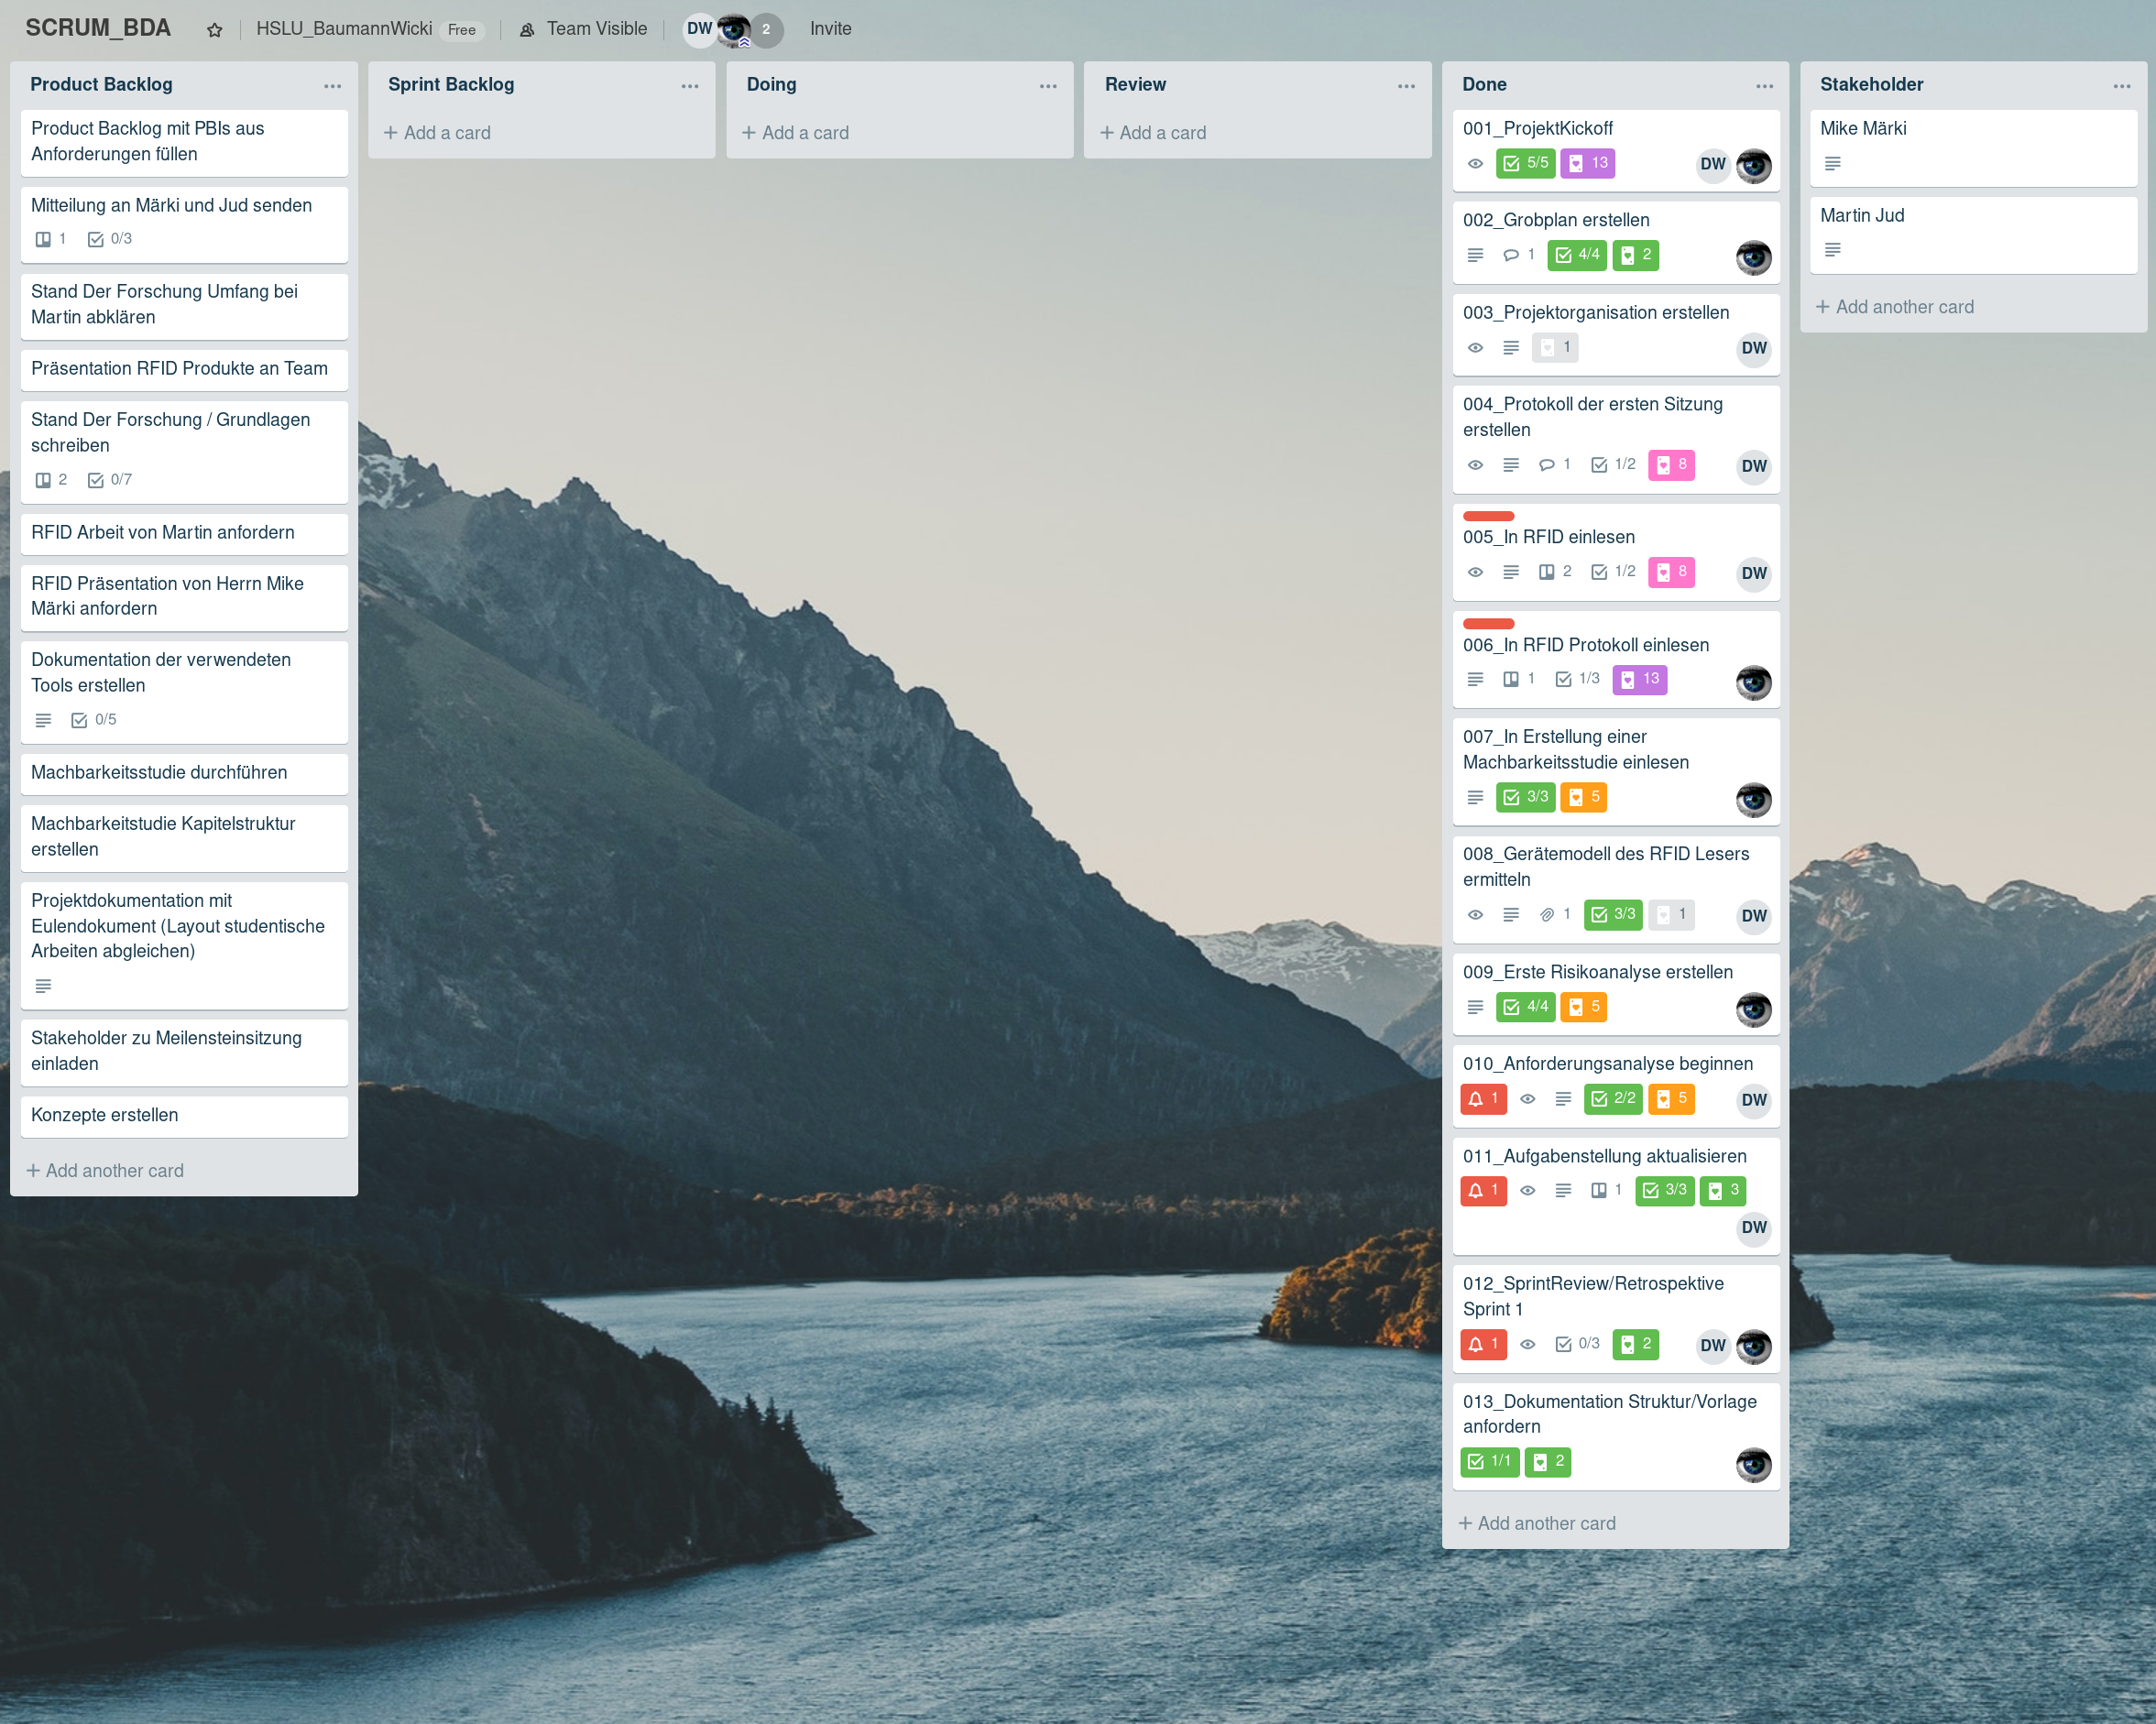
\includegraphics[height=0.9\textheight,keepaspectratio]{Sprint01_Review_Sprint02_Planning.png}
\end{landscape}

\newpage
\section*{Sprint02 Review}
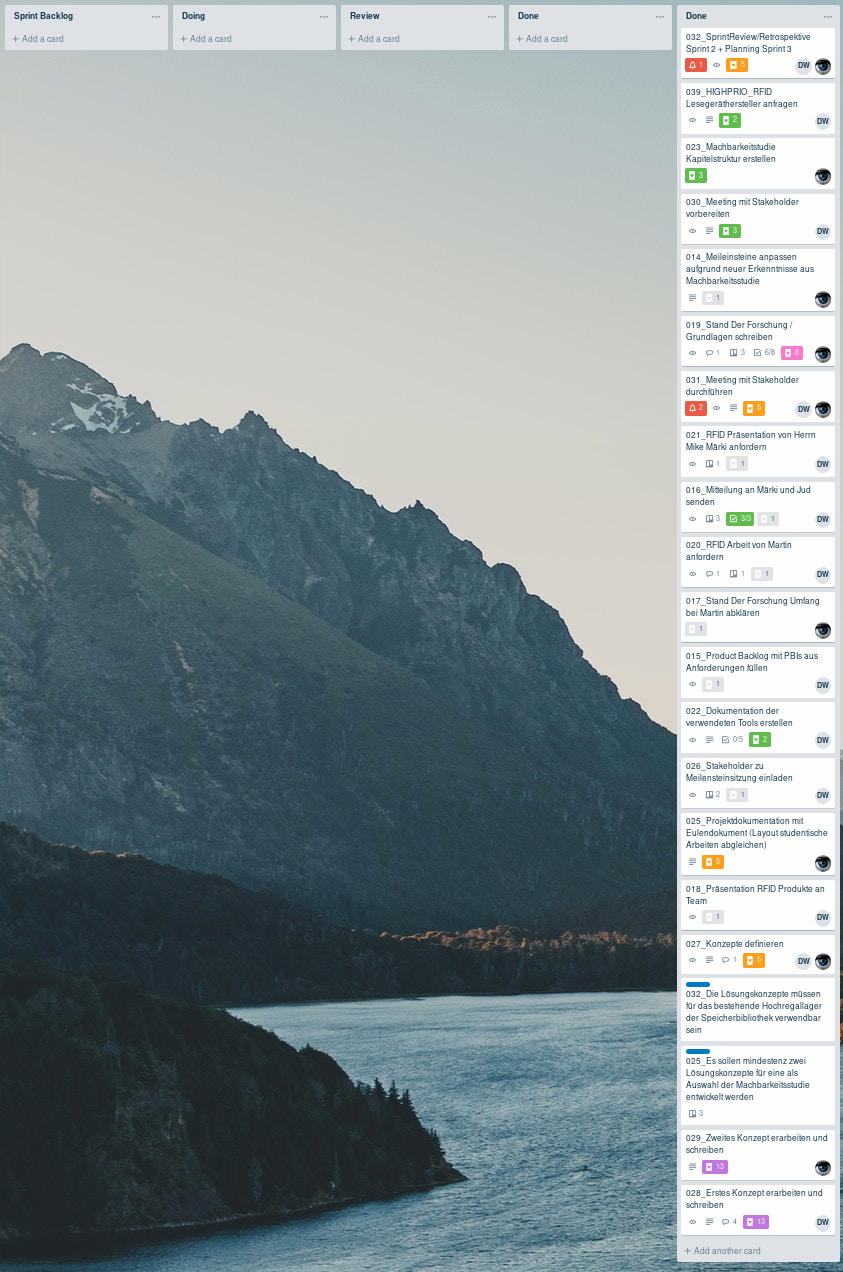
\includegraphics[height=0.9\textheight,keepaspectratio]{Sprint02_Review.png}

\newpage
\begin{landscape}
	\section*{Sprint03 Planning}
	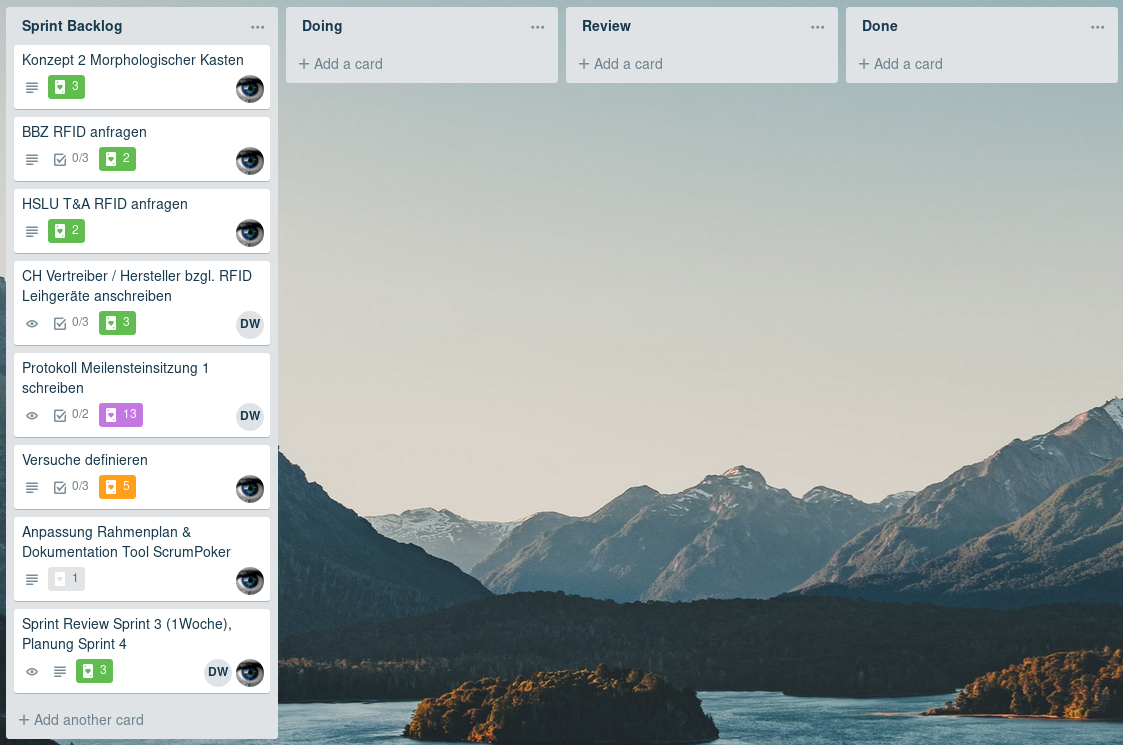
\includegraphics[height=0.9\textheight,keepaspectratio]{Sprint03_Planning.png}
\end{landscape}

\newpage
\section*{Sprint03 Review}
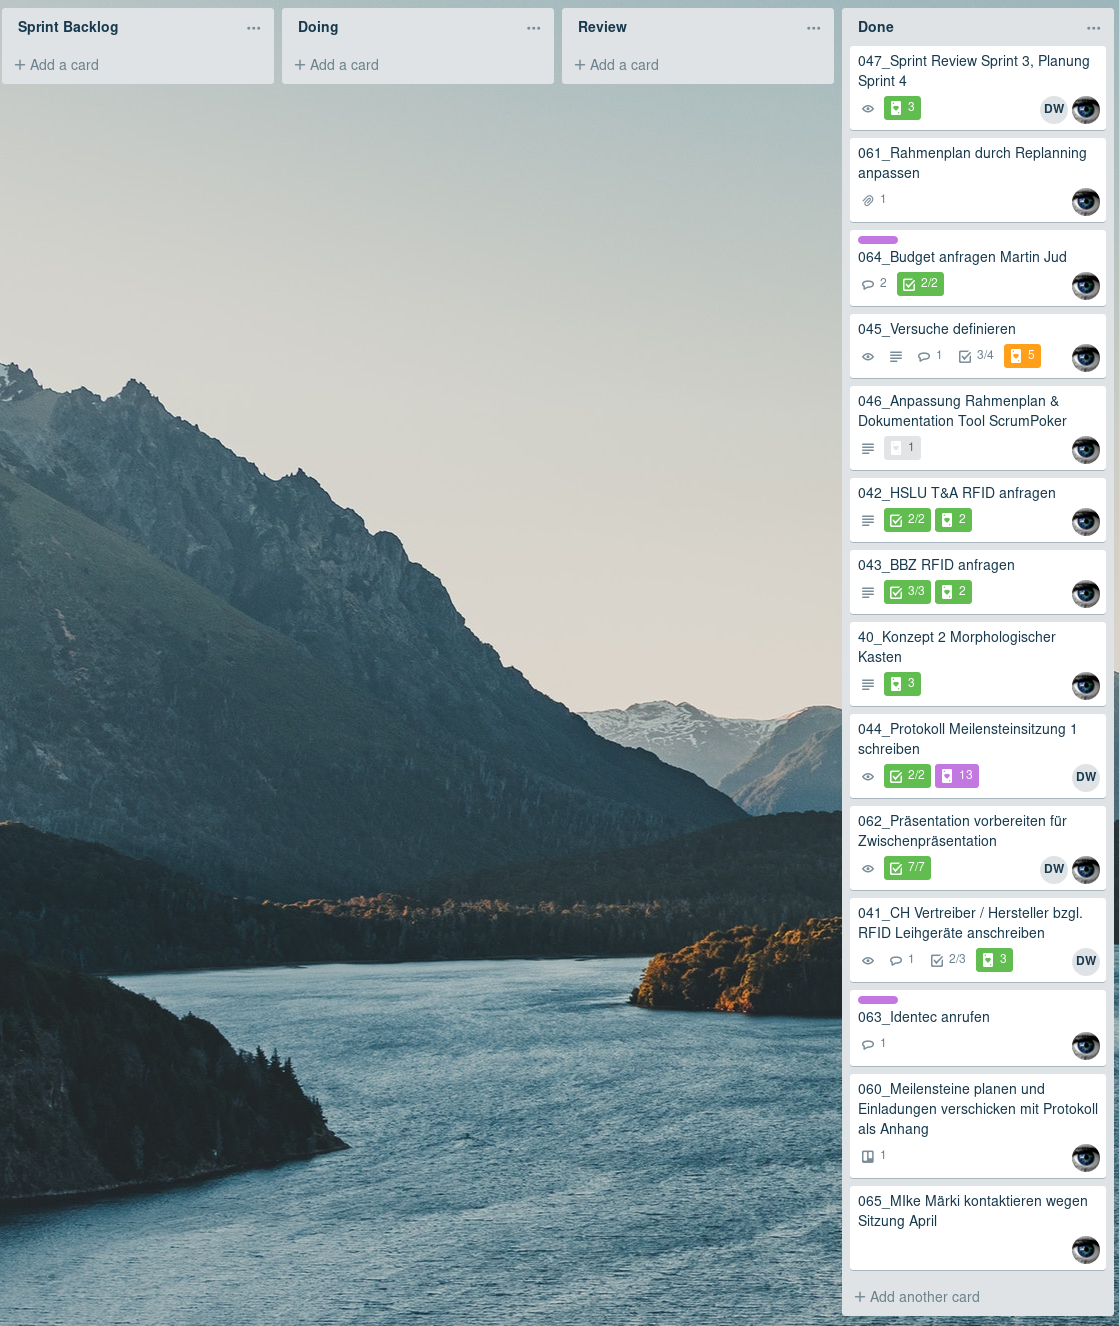
\includegraphics[width=\linewidth,keepaspectratio]{Sprint03_Review.png}

\newpage
\begin{landscape}
	\section*{Sprint04 Review}
	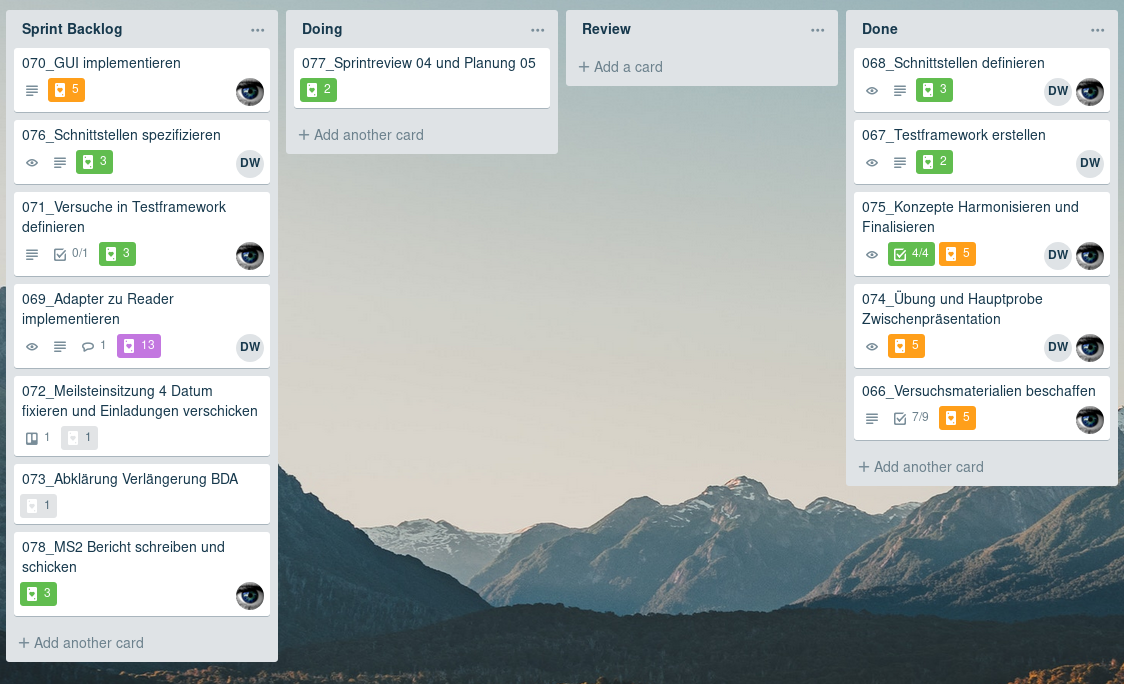
\includegraphics[height=0.9\textheight,keepaspectratio]{Sprint04_Review.png}
\end{landscape}

\newpage
\section*{Sprint05 Planning}
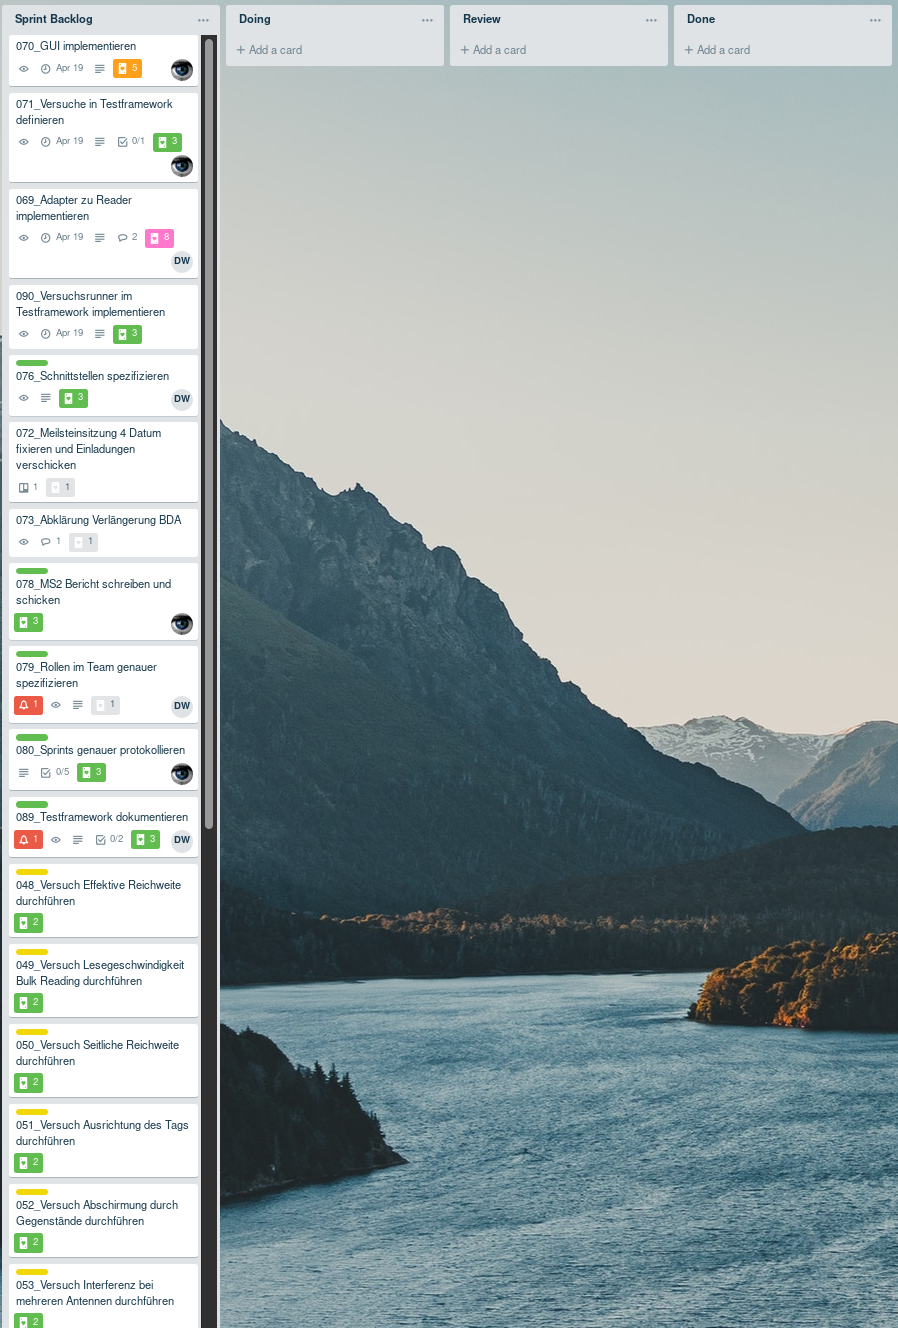
\includegraphics[width=0.9\linewidth,keepaspectratio]{Sprint05_Planning_01.png}
\newpage
\noindent
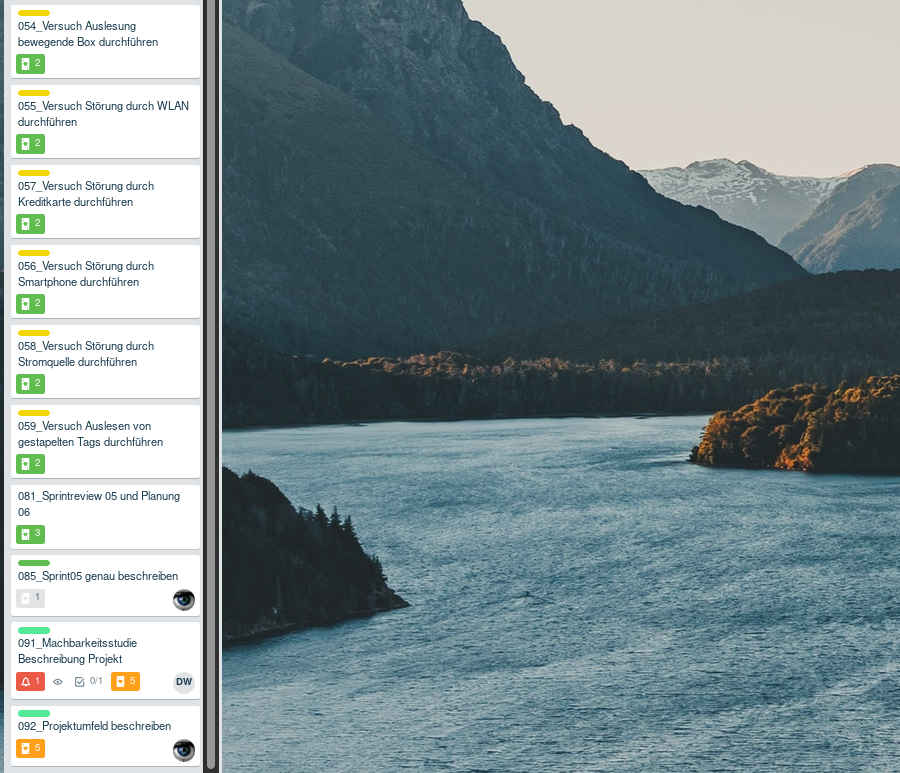
\includegraphics[width=0.9\linewidth,keepaspectratio]{Sprint05_Planning_02.png}

\newpage
\section*{Sprint05 Review}
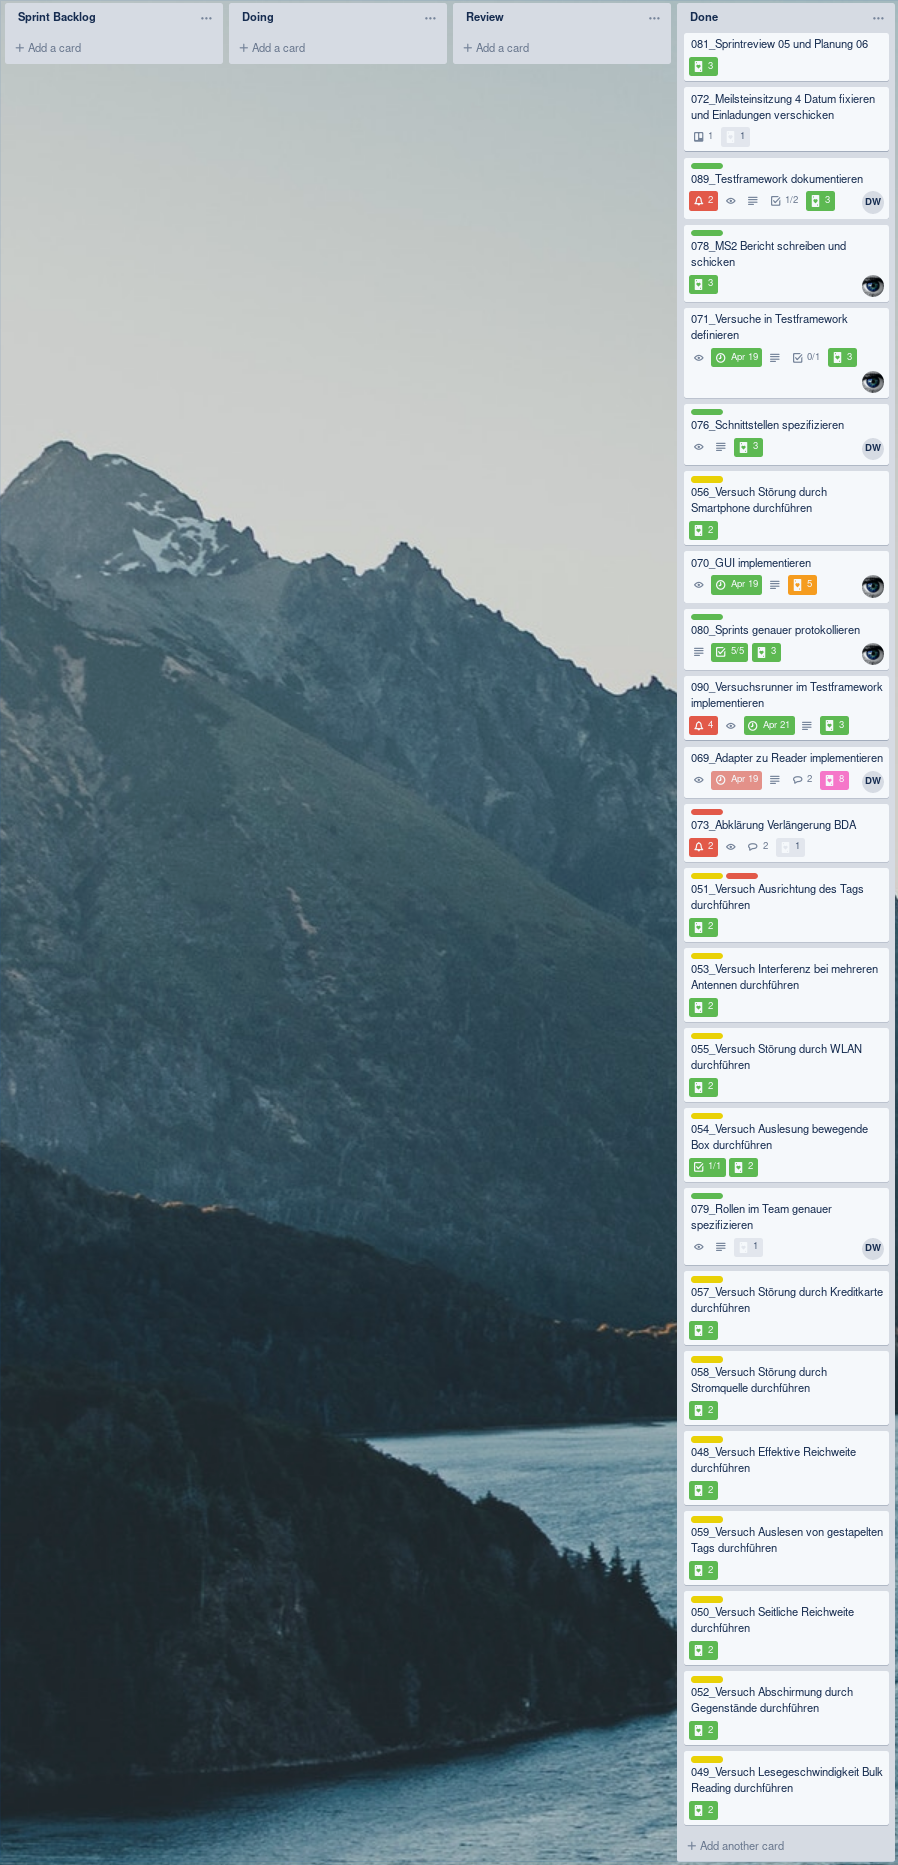
\includegraphics[height=0.95\textheight,keepaspectratio]{Sprint05_Review.png}

\newpage
\section*{Sprint06 Planning}
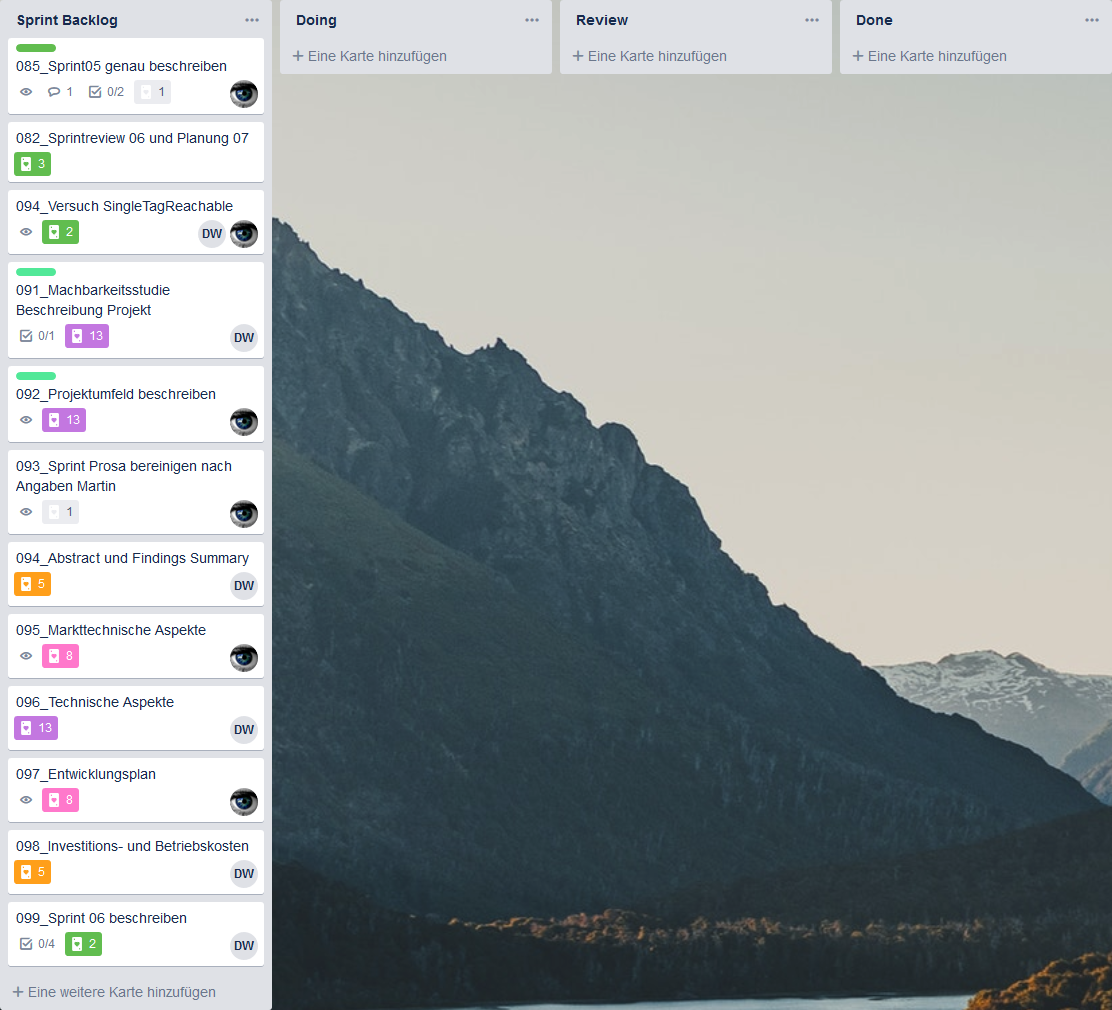
\includegraphics[width=0.9\linewidth,keepaspectratio]{Sprint06_Planning.png}


\end{document}
